% Literature Review
% 01/03/11
% (Use \include{filename} in diss proposal file

\documentclass[a4paper,12pt]{report} 	% report used for dissertations

\usepackage{anysize} 		% allows me to set margins
\usepackage{indentfirst}
\usepackage{apacite}		% for apa style
\usepackage{graphicx}		% for graphics
\usepackage{times}
\usepackage{mathtools}
\usepackage{textcomp }

\marginsize{1.5in}{1.5in}{1.25in}{1.25in}	% left, right, top, bottom
\linespread{2}					% double-spacing
\begin{document}

\pagenumbering{arabic}

\begin{flushleft}			% generates left-aligned paragraphs
\setlength{\parindent}{30pt}	% This starts every paragraph with an indent

\section*{Chapter 3} % * suppresses heading numbers	
\noindent {\Huge Methods}
\subsection*{3.1 System Design}
\subsubsection*{3.1.1 Languages and Interoperability}
By relying on the many years of development, user-feedback, and re-development of commercial audio-implementation systems to provide the appropriate level of abstraction necessary for an efficient GP search (as discussed in the Prior Work above), we have decided to apply GP directly within one of these audio-implementation systems. While those previously listed would all be good candidates for evolving synthesis algorithms, Max (developed by \emph{Cycling '74}) is chosen because, as pointed out by Lazzarini, ``MaxMSP and its variants have lately become the most used of these systems, because of their user-friendliness'' (2004, p. 356). Lazzarini's statements have two implications. First, due to Max's popularity, the resultant algorithms (i.e. Max patches) output from our system will be available to more composers. Second, due to Max's ease of use, the algorithms will automatically be accompanied by interfaces for timbre exploration that are accessible to the non-technically oriented composer, whom this research will benefit most.

While it would be possible to design the entire system in Max by utilizing either Java via the \emph{mxj} object or JavaScript via the \emph{js} object for the implementation of the GP framework, the timbre feature extraction, and the timbre similarity calculation code, we have decided to use Python for the 'heavy lifting' instead. The main reason for this choice is that Python has an extensive set of third-party libraries developed for it in the domains of machine learning, artificial intelligence, music information retrieval, etc. that allow for rapid development of all the necessary code used for timbre extraction and similarity calculations. It also has popular linear algebra libraries (numpy, scipy) and a popular and easy-to-use graphing framework (matplotlib) that may be utilized throughout the codebase to simplify calculations and produce figures exhibiting our experimental results.

Therefore, we have implemented all genetic programming code, which includes both the fitness function calculation and the genetic operator applications that follow in Python. This means that the only processing required of Max is the actual patch creation (within the Max environment) and the signal processing that follows.

The problem with choosing a language that does not directly interface with Max, which is the case with Python, is that a translation layer must be inserted between Max and the chosen language so that they can communicate appropriately. Given the tasks assigned to Python and those assigned to Max, one may observe that this communication can be described as follows:
\begin{enumerate}
\item Python communicates to Max what patch to generate, including all objects and connections between object inlets and outlets. 
\item Max communicates to Python the `results' of its signal processing through the generated patch.
\end{enumerate}
The first item is handled using a JavaScript translation layer, where Python translates its internal representation of a Max patch into JavaScript code, which the Max js object immediately runs to generate the desired Max patch (see Figure 1). 
\begin{figure}[h!]
\begin{center}
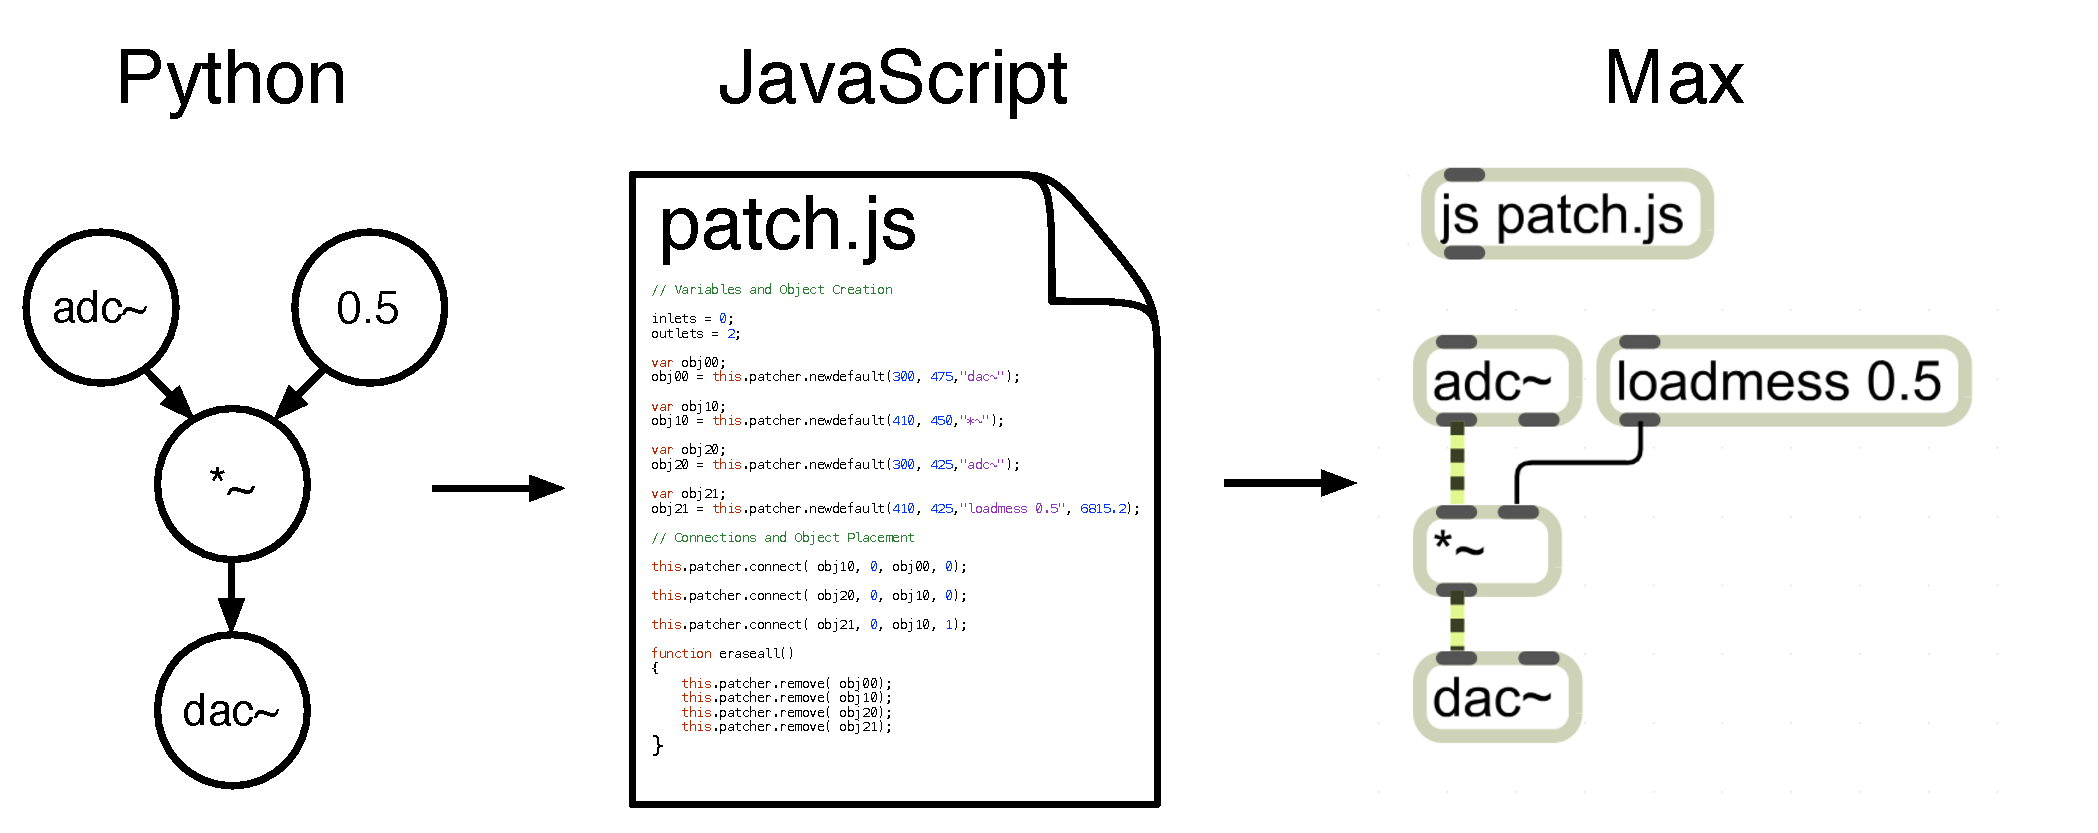
\includegraphics[scale=0.4]{JSTranslation}
\caption[Generating a Max patch given a parse-tree]{Translation of a Python `MaxPatch' into an equivalent patch in Max via JavaScript.}
\end{center}
\end{figure}
\\
The second item is handled by requiring Max to write the audio at the output of a given Max patch to a file, which is then read  by Python and used for the timbre feature calculation (see Figure 2).
\begin{figure}[h!]
\begin{center}
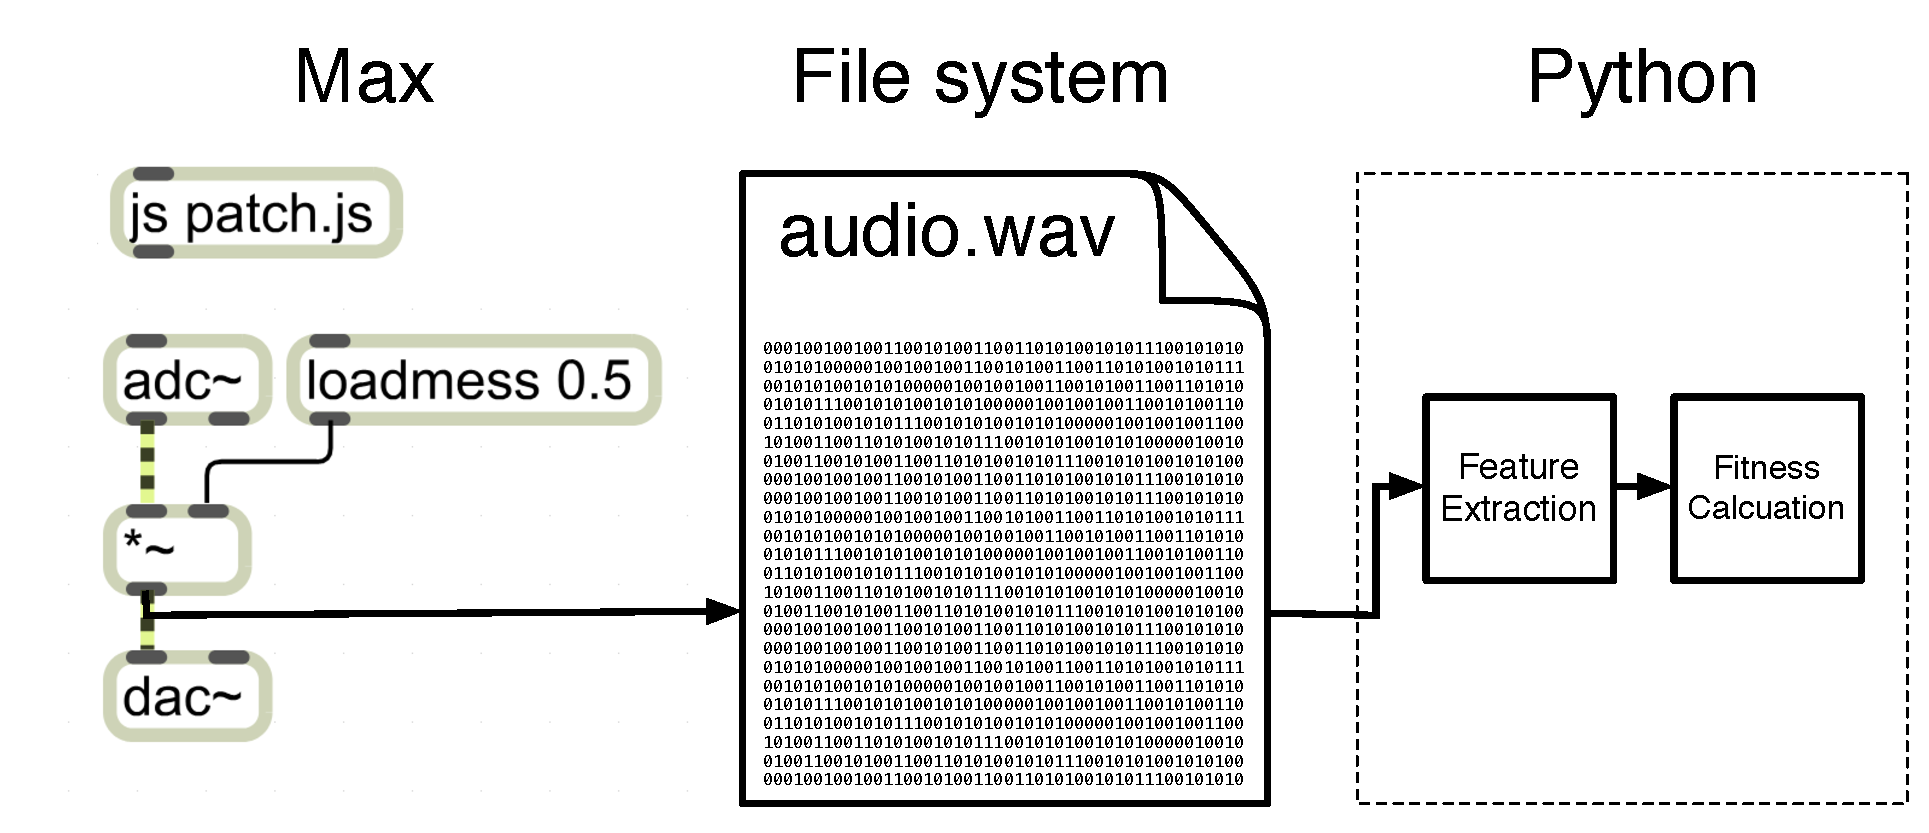
\includegraphics[scale=0.4]{MaxAudioToPython}
\caption{Writing audio output from a Max patch to a wav file that is then read and processed by Python code.}
\end{center}
\end{figure}
\\
In order for Python to have an internal representation of Max patches, we have mirrored all Max constructs using Python classes. For example, we have written MaxPatch, MaxObject, MaxInlet, and MaxConnection classes that represent patches, objects, inlets, and connections in Max. Therefore, the initial population creation is done in Python, the resultant patches are translated into JavaScript commands that, via Max's js object, are run in Max to generate the corresponding Max versions of the patches, an audio signal (more on this later) is sent through the patch, the output is recorded to a file, and Python reads in the file and uses its contents to calculate the fitness of the corresponding patch that produced it in order to apply genetic operators and create the next generation of patches.

\subsubsection*{3.1.2 Framing as a Genetic Programming Problem}
The majority of GP research uses tree data structures to represent each individual algorithm within a population. We have adopted this representation in evolving Max patches that function as synthesis algorithms. Since Max, in general, allows the creation of graph structures, we have decided to limit the number of possible patch representations by enforcing several rules. 
\begin{enumerate}
\item The root of each tree will be Max's audio output object (the \emph{dac\texttildelow{}}), internal nodes will represent other Max objects are able to receive Max signal input and return Max signal output, and the leaf nodes or terminals will represent either audio generators (including audio playback objects and live audio input objects) or input parameters to the patch (see fig. 3).
\begin{figure}[h!]
\begin{center}
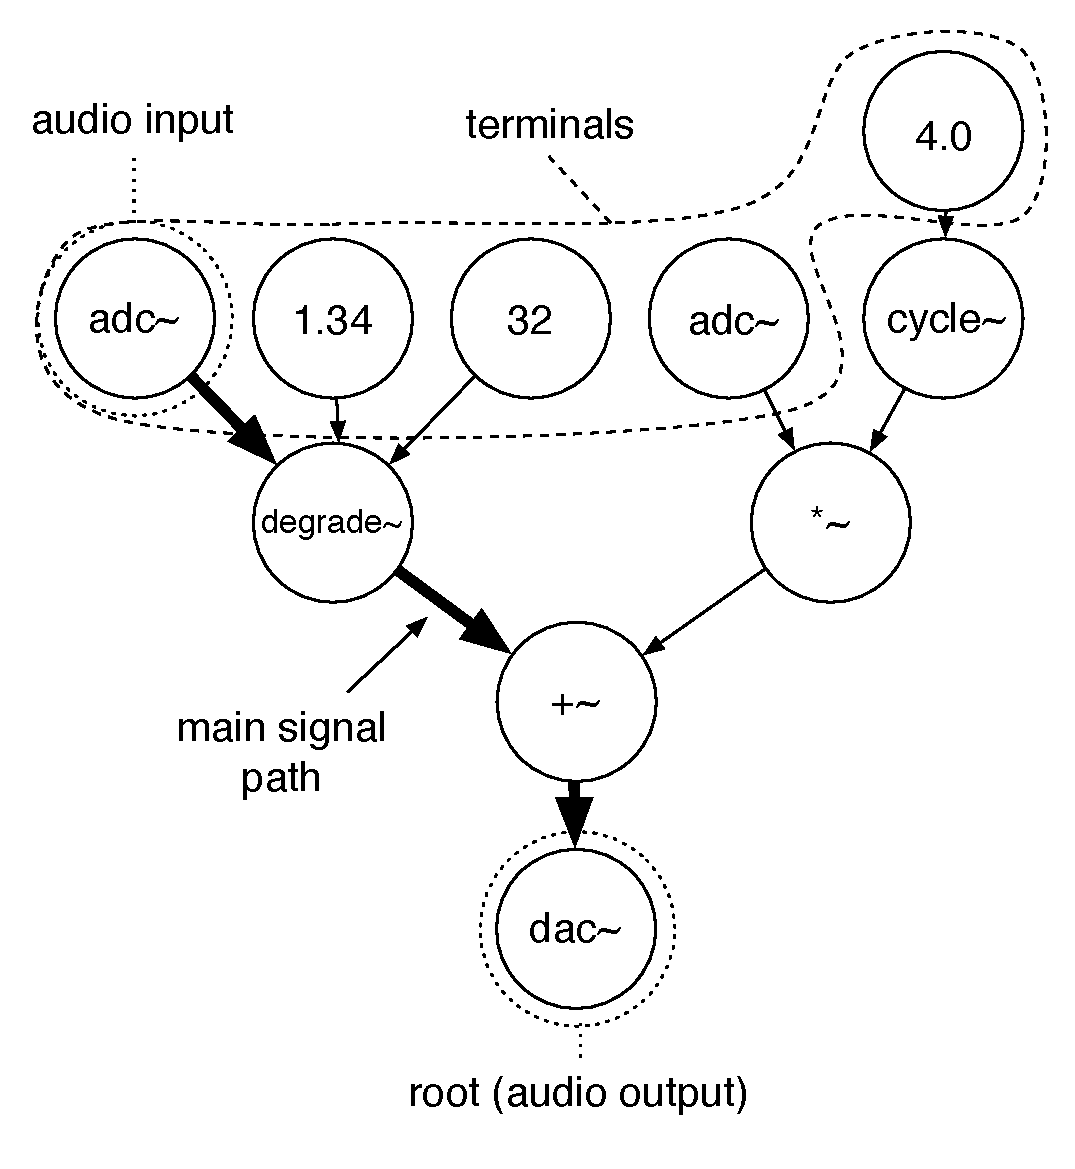
\includegraphics[scale=0.7]{RootTree}
\caption{An example Max patch represented as a directed tree with the audio signal flowing from patch's terminals towards its root.}
\end{center}
\end{figure}
\\
\item By ensuring that at least one terminal is an audio generator, a main signal path can be traced from the input object to the \emph{dac\texttildelow{}}, as seen in Figure 3. Therefore, the patch can be similarly viewed as a black box with audio going in and audio coming out---the fundamental representation of a synthesis algorithm. If more than one audio generator is chosen as a terminal, any could be viewed as that which produces the main signal path, while all others can be regarded as audio-rate input parameters to the system. Thus, the black box representation still holds.
\end{enumerate}

It should be noted that adhering to the above rules will restrict the search space over all Max patches. Any time such a search space restriction is put in place, one must make sure viable solutions are not left out of the resultant subspace over with the search will occur. Our goal is to search over the space of all synthesis algorithms and not over all Max patches (which occupies a much larger space), so as long as we can be sure that the above restrictions do not leave out any synthesis algorithms, we can proceed without worry.

Any Max patch can be easily be represented by a finite set of directed acyclic graphs (DAGs) - where directed edges correspond to Max connections with direction pointing from object outlet to object inlet and vertices correspond to Max objects (see Figure 4).
\begin{figure}[h!]
\begin{center}
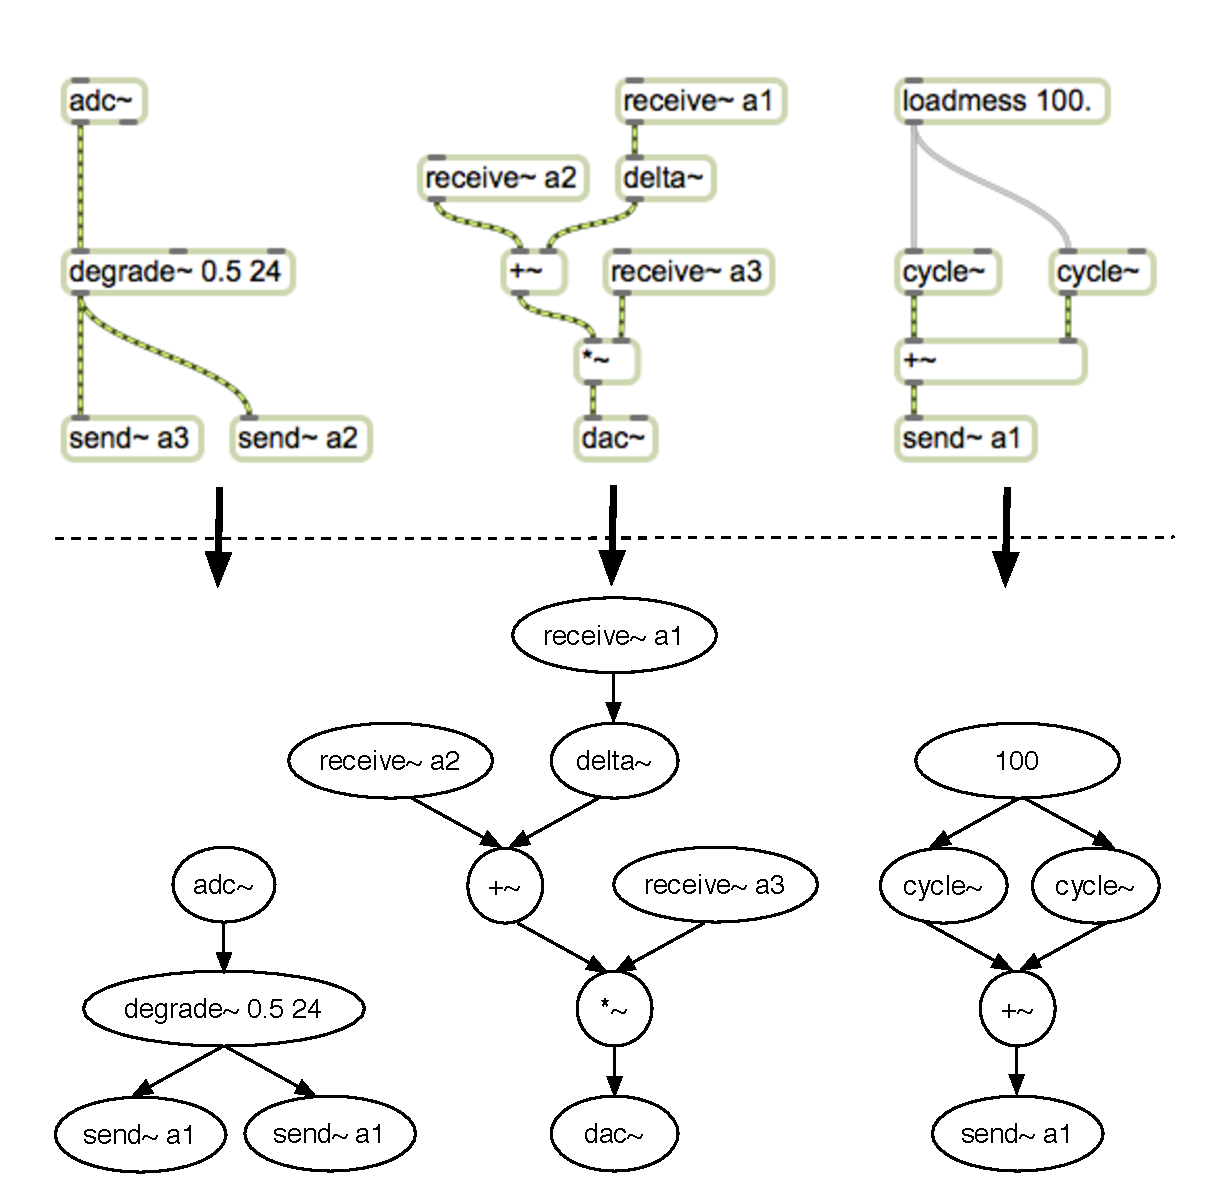
\includegraphics[scale=0.7]{MaxDAGs}
\caption{A Max patch and its corresponding representation as a set of DAGs}
\end{center}
\end{figure}
\\
In the case that a Max object would exist in a patch with arguments (as pictured in Figure 5) and no inputs attached to the inlets whose initial values are represented by those arguments, we can replace it with its default version (i.e. one without arguments) and with a set of connected \emph{loadmess} objects supplying those arguments and acting as terminals, thereby transforming a patch containing objects with arguments and exposed inlets to one with a more direct correlation to a set of DAGs.
\begin{figure}[h!]
\begin{center}
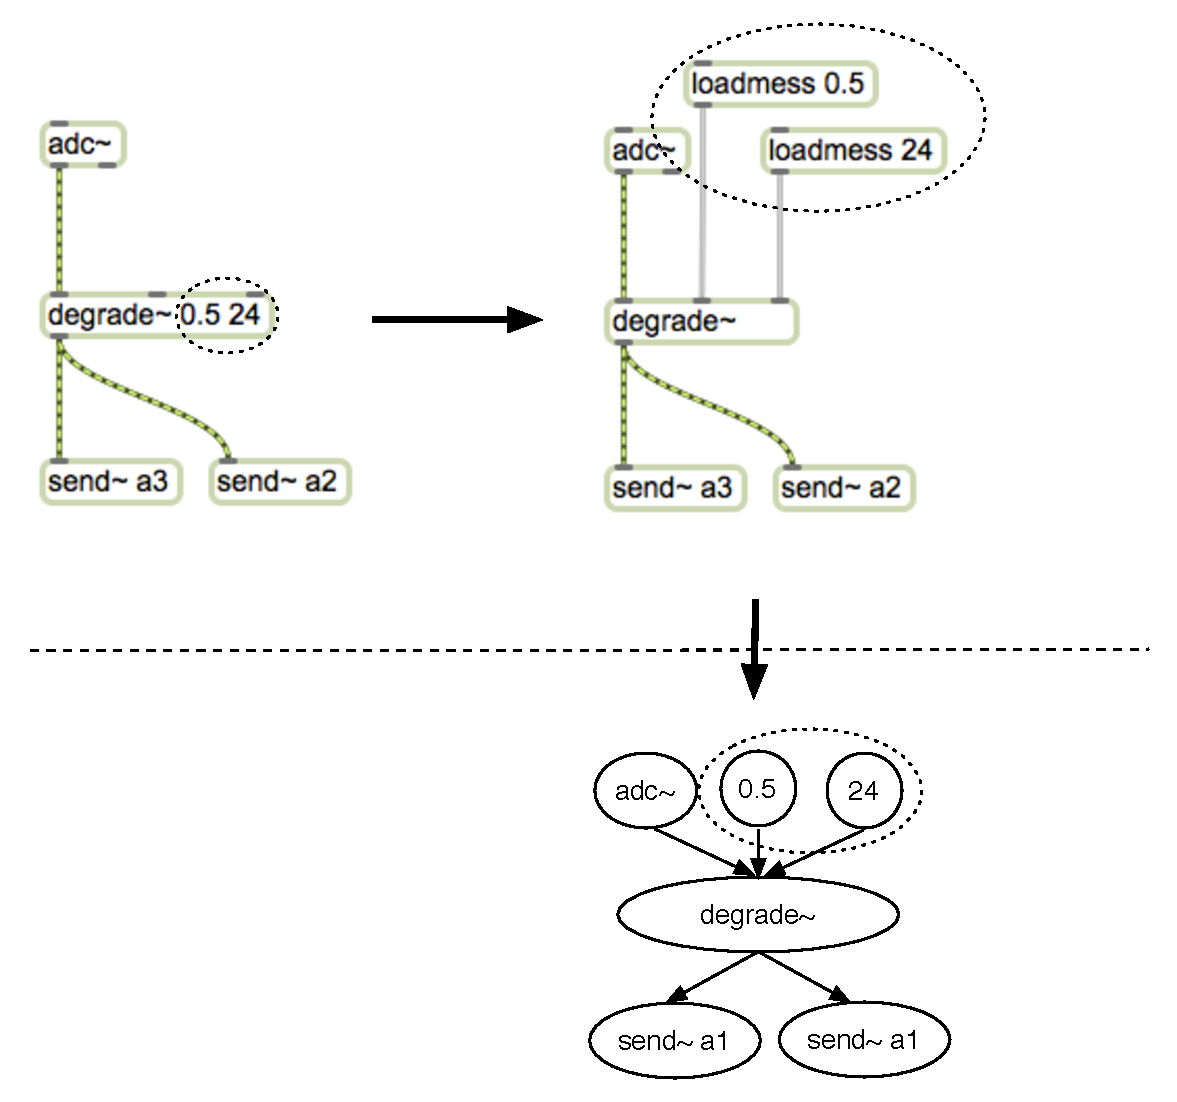
\includegraphics[scale=0.8]{MaxDAGsLoadmess}
\caption{The same \emph{degrade\texttildelow{}} object in two Max patches (one with arguments and one with load mess objects).}
\end{center}
\end{figure}
\\
Max objects come in a number of flavors with regard to what type of data can flow into and out from their connections. The objects that we are primarily interested in are Max's signal processing objects, which output Max's signal data type (i.e. data produced, transformed, and output at the patch's audio sample rate). While Max does provide mechanisms by which to convert from its other data types (e.g. matrices of video data, MIDI control rate data) to the signal data type, our research will focus only on the set of objects designed specifically to work with audio data. The terminating Max signal processing object for audio output via an audio device is the \emph{dac\texttildelow{}}. Since any signal processing algorithm must terminate at an output node of this type, the \emph{dac\texttildelow{}} will be required of any patch we wish to search over. If there is only one \emph{dac\texttildelow{}} in the patch, then only the objects in its directed acyclic graph will contribute to what is sent to the audio output device, unless there is another directed acyclic graph that terminates with a \emph{send} or \emph{send\texttildelow{}} object that passes data to a \emph{receive} or \emph{receive\texttildelow{}} object within the same DAG as the \emph{dac\texttildelow{}}. However, in this case, the send to receive connection could easily be represented by a directed edge and therefore we are still left with only one DAG with a \emph{dac\texttildelow{}} (see Figures 6 and 7).
\begin{figure}[h!]
\begin{center}
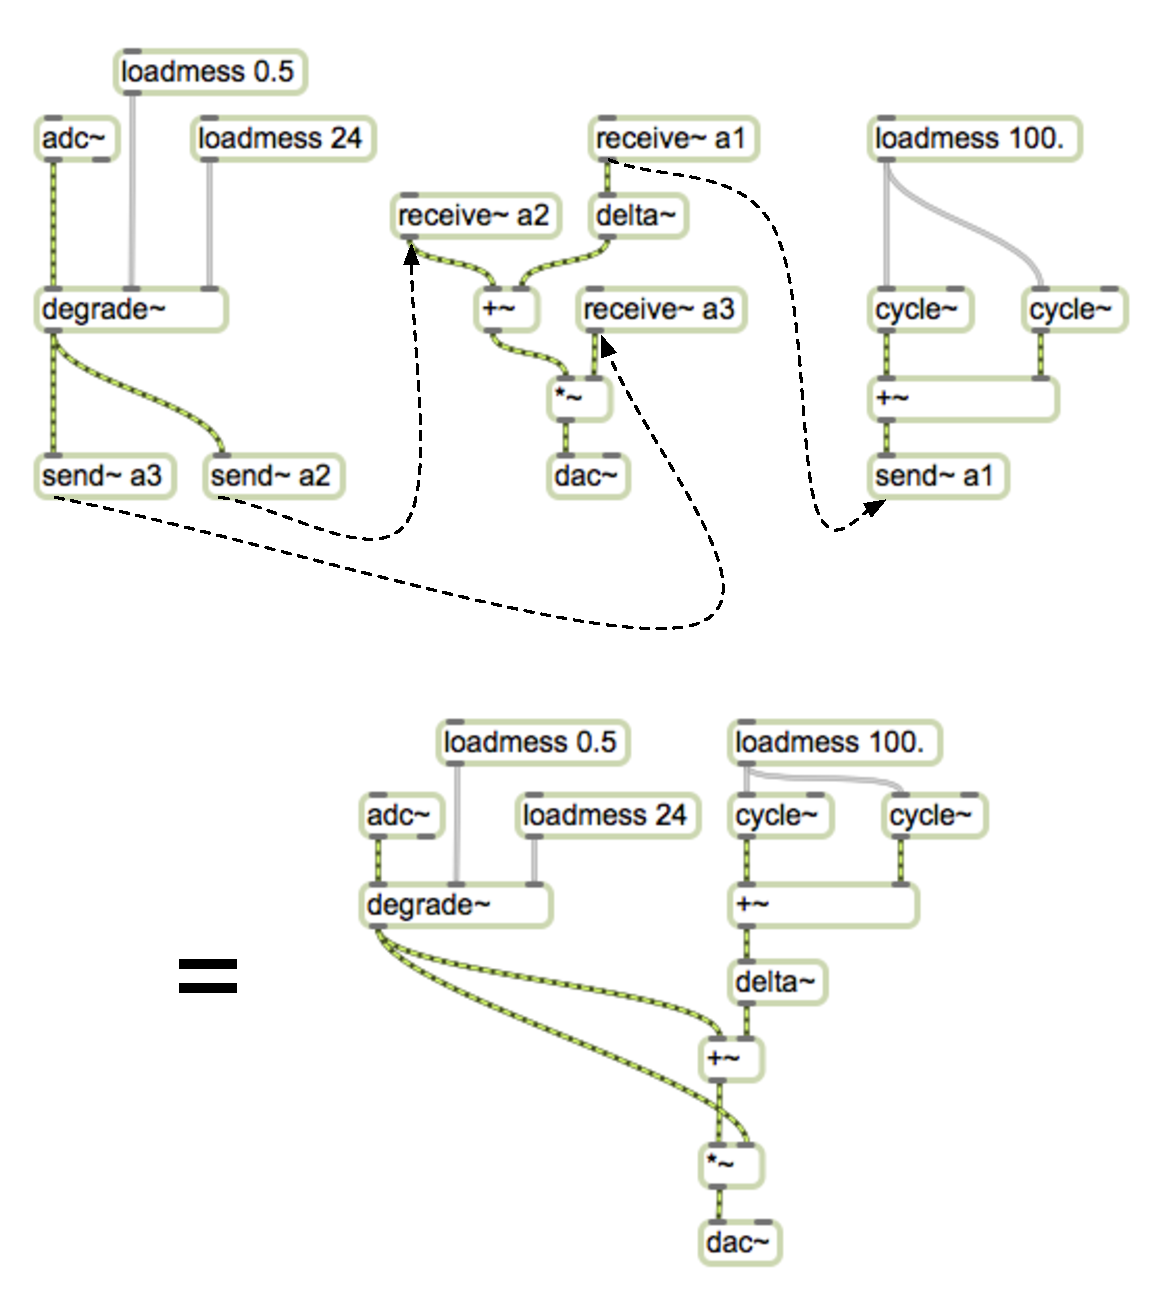
\includegraphics[scale=0.75]{MaxDAGsSendReceive1}
\caption{The original Max patch from Figure 4 replaced by its equivalent patch without send\texttildelow{} or receive\texttildelow{} objects.}
\end{center}
\end{figure}
\begin{figure}[h!]
\begin{center}
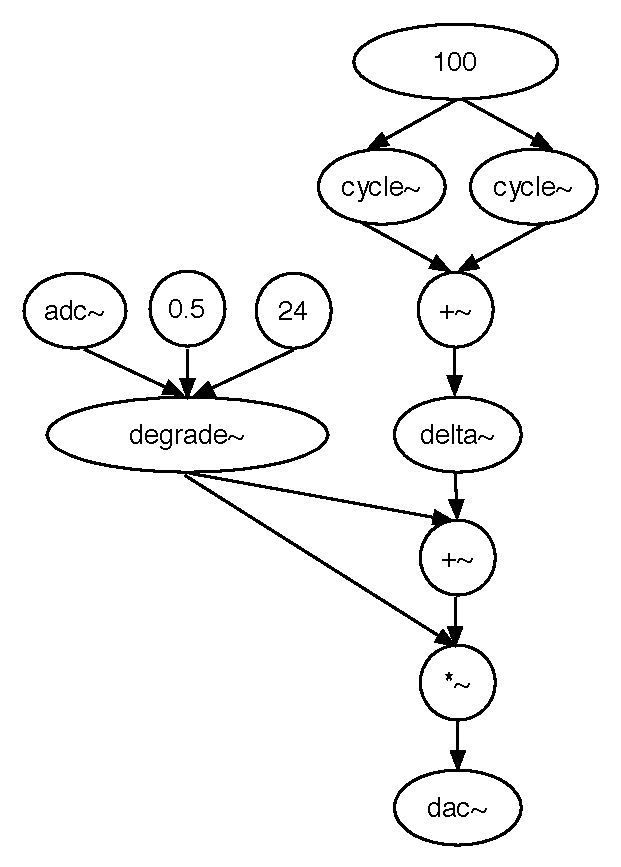
\includegraphics[scale=0.8]{MaxDAGsSendReceive2}
\caption{The single DAG representation of the reduced patch in Figure 6.}
\end{center}
\end{figure}
\\
If there are two or more \emph{dac\texttildelow{}} nodes in the DAG, the signals sent to them are simply summed before being sent to the audio output device. Therefore, we could easily model the same DAG with one \emph{dac\texttildelow{}} and one or more \emph{+\texttildelow{}} objects to sum all paths that would be summed by Max automatically (see Figure 8). 
\begin{figure}[h!]
\begin{center}
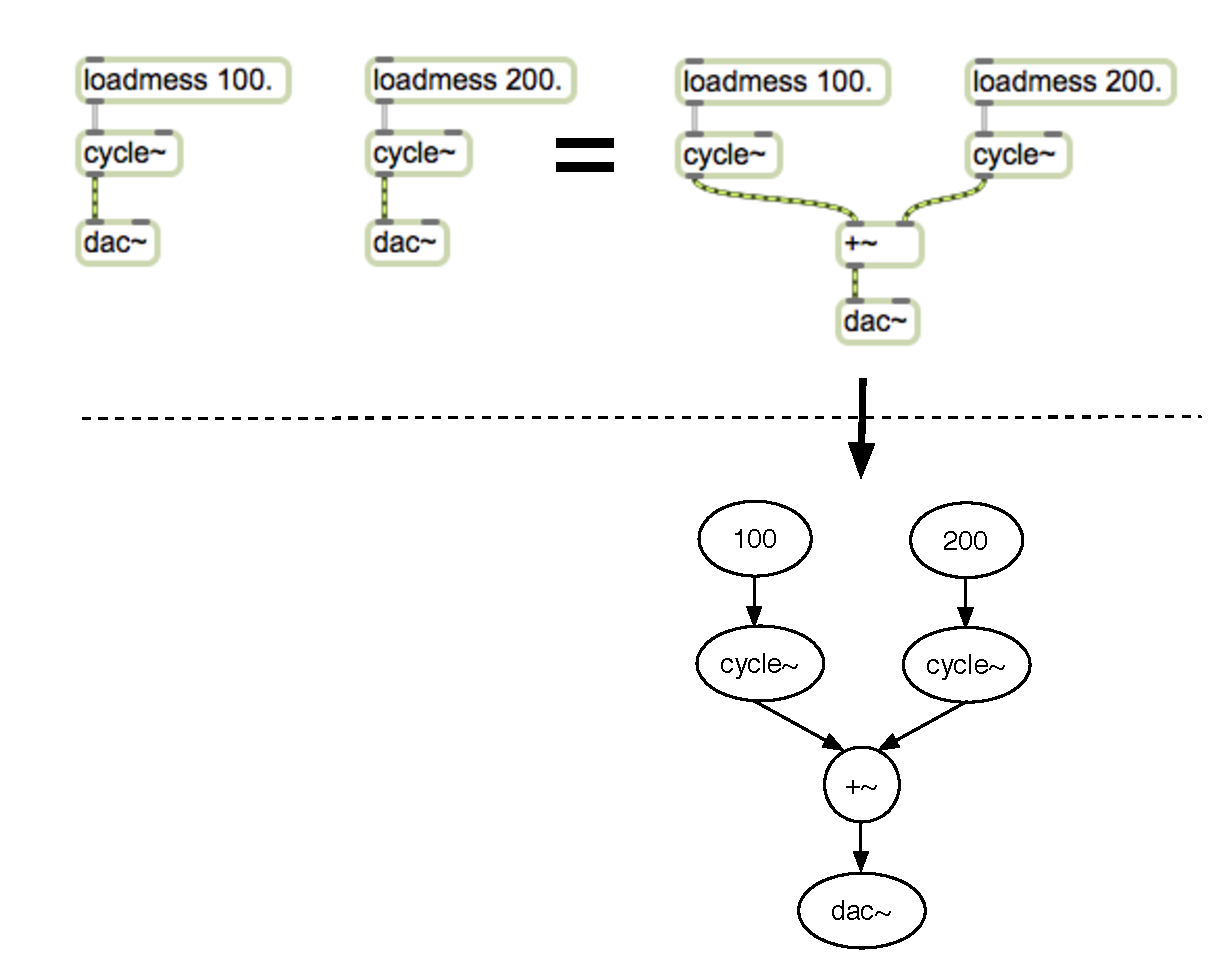
\includegraphics[scale=0.7]{MaxDAGs2DACs}
\caption{A single DAG representation of a Max patch with two \emph{dac\texttildelow{}} objects.}
\end{center}
\end{figure}
\\
Therefore, the only difference between the representation we've determined all signal processing Max patches can be reduced to and the tree data structure we are using to represent all patches within Python that we search over is that a tree data structure cannot have internal crossed paths. In other words, given two vertices u and v in our tree representation, there is at most one possible path connecting u and v. This is not the case for the DAG representation of all possible synthesis algorithms in Max that we have arrived at given the above arguments (see Figure 9 for an example).
\begin{figure}[h!]
\begin{center}
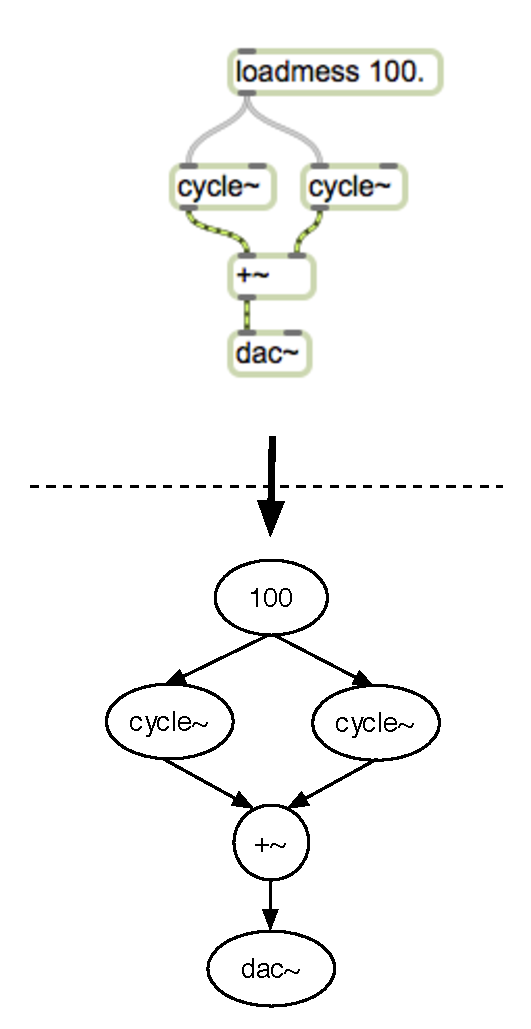
\includegraphics[scale=0.8]{MaxDAGsCrossedPaths}
\caption{A simple Max patch whose DAG representation has crossed paths and therefore is not a tree.}
\end{center}
\end{figure}
\\
However, for every possible DAG representation discussed, there is an equivalent tree representation that can be obtained by splitting each crossed path, duplicating all nodes below it (or 'above' it in the visual diagrams presented) for each node at the end of the crossed path (see Figure 10).
\begin{figure}[h!]
\begin{center}
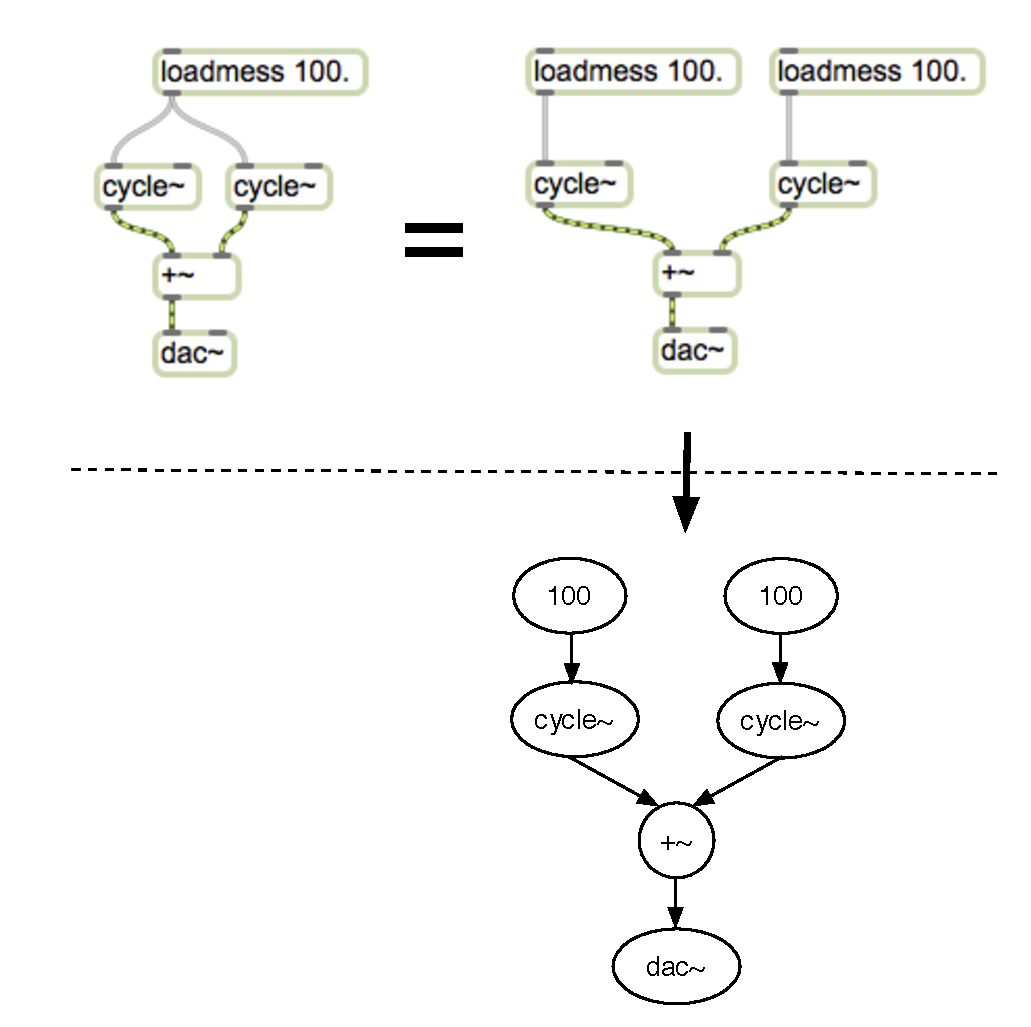
\includegraphics[scale=0.8]{MaxDAGsCrossedPaths2}
\caption{The same Max patch with crossed paths from Figure 9 and its equivalent Max patch with a tree representation.}
\end{center}
\end{figure}
\\
Taking all of the above arguments into account it is clear that by choosing the tree representation we have (which is necessary to leverage most work in the GP domain) we are not excluding Max synthesis topologies. 

It should also be noted that starting with a random tree representation of a Max patch can lead to patches that are not syntactically correct. Our trees are only valid representations of Max patches if their edges represent connections that are allowed in the Max environment. In other words, connections to inlets are valid only if the data flowing over those connections are accepted by the inlets. Therefore, syntactic correctness must be enforced while searching over the input-space defined by these trees. As previously noted in the discussion of strongly-typed GP, enforcing data type constraints during search is a simple way to disregard invalid topologies and make the search much more efficient without excluding possible solutions. We have therefore decided to incorporate knowledge of Max syntax into our system.

Information regarding syntactic correctness rules in Max is supplied to Python via a text file, which contains a list of Max object names, each followed by their respective inputs' accepted data types and reasonable input ranges, and their output data type (see Figure 11).
\begin{figure}[h!]
\begin{center}
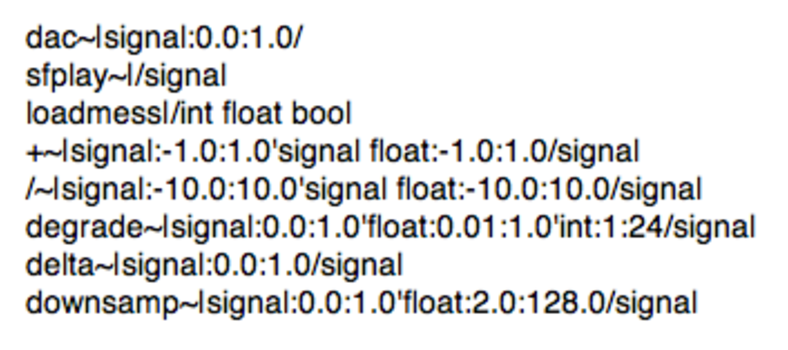
\includegraphics[scale=0.8]{SyntaxInfo}
\caption{Example of the object\_list.txt file that contains syntax information for the various objects used to generate patches with our system.}
\end{center}
\end{figure}
\\
The format is as follows where the inlet information is simply repeated for multiple inlets and the output type is repeated for multiple outlets (with spaces in between outlet types as shown in Figure 11):
\\
\textbf{\emph{objectName\textbar inlet1InputType:minVal:maxVal'.../outletType1 ...}}

`Reasonable ranges' must be chosen carefully as to not be too restrictive, since a particular object may be required to function outside of what is considered its norm in order to contribute to the best solution. Therefore, one of the variables we have decided to modify throughout our experiments are the sizes of the reasonable ranges for each object used. Even more importantly, it should be noted that the number of unique Max objects available for use in our system (and therefore the size of the patch space searched) is limited by how many objects we provide syntactic information for. Therefore, we have also investigated how our system performs by varying the number of objects in an attempt to determine whether a general set exists that is small enough for the search to provide a good solution over a reasonable amount of iterations, but also large enough to provide a solution that produces content that similar enough to the target to be considered a success. Specifics around the variation of both accepted inlet value ranges and object sets are provided in the Experiment Design section below.

By representing synthesis algorithms using the tree representation discussed above, the input space can be viewed as a set of such tree topologies, where each point in the space corresponds to a topology with a unique set of parameters and objects. This representation is the common representation for most GP systems and we can therefore leverage much of the research carried out in this field in order to produce an effective system.

\subsubsection*{3.1.3 Genetic Programming System Overview}
The GP system that we have designed follows the typical GP blueprint at a high level. We will provide a brief overview of the mechanisms involved in such a system and then will discuss where we have chosen to experiment and in what ways. A more detailed treatment of Genetic Programming can be found in John Koza's book \emph{Genetic Programming: On the Programming of Computers by Means of Natural Selection} (Koza, 1992).

As mentioned in \textbf{Chapter 2 - Prior Work}, Genetic Programming is a parallel search technique; meaning that instead of starting by looking in one location in space and moving along some search path from there, Genetic Programming starts looking in many places at once and allocates more resources to those regions that show promise. The search process loosely models biological evolution and so borrows a number of terms from that domain. The number of points in algorithm space searched over at each iteration is defined as the current \emph{population}, with the first iteration starting with an initial population. The objective function that one wants to maximize over the search is referred to as the \emph{fitness function} and each successive iteration favors regions of space with higher fitness as it \emph{selects} individuals for the next \emph{generation} to \emph{mutate} and effectively `mate' in a process where algorithms swap pieces of their code in a process called \emph{crossover}. 

There are many variations of the operations (known as \emph{genetic operators}) used to \emph{evolve} algorithms from generation to generation and also the selection criteria for the algorithms that are subjected to these operations. The fitness function is problem-dependent and the quality of the solutions found using GP is completely dependent on how well it models the actual fitness of each algorithm with respect to the stated goal. Our efforts in evolving Max patches have led us to explore all facets of GP in depth and we have found, as will be detailed in \textbf{Chapter 4 - Results}, that varying some meta-parameters have a large impact on solution quality, while others seem to have very little. Figure 12 shows a high-level flow diagram of our GP system with components marked off by what sub-sections in \textbf{3.2 Experiment Design} they are discussed.
\begin{figure}[h!]
\begin{center}
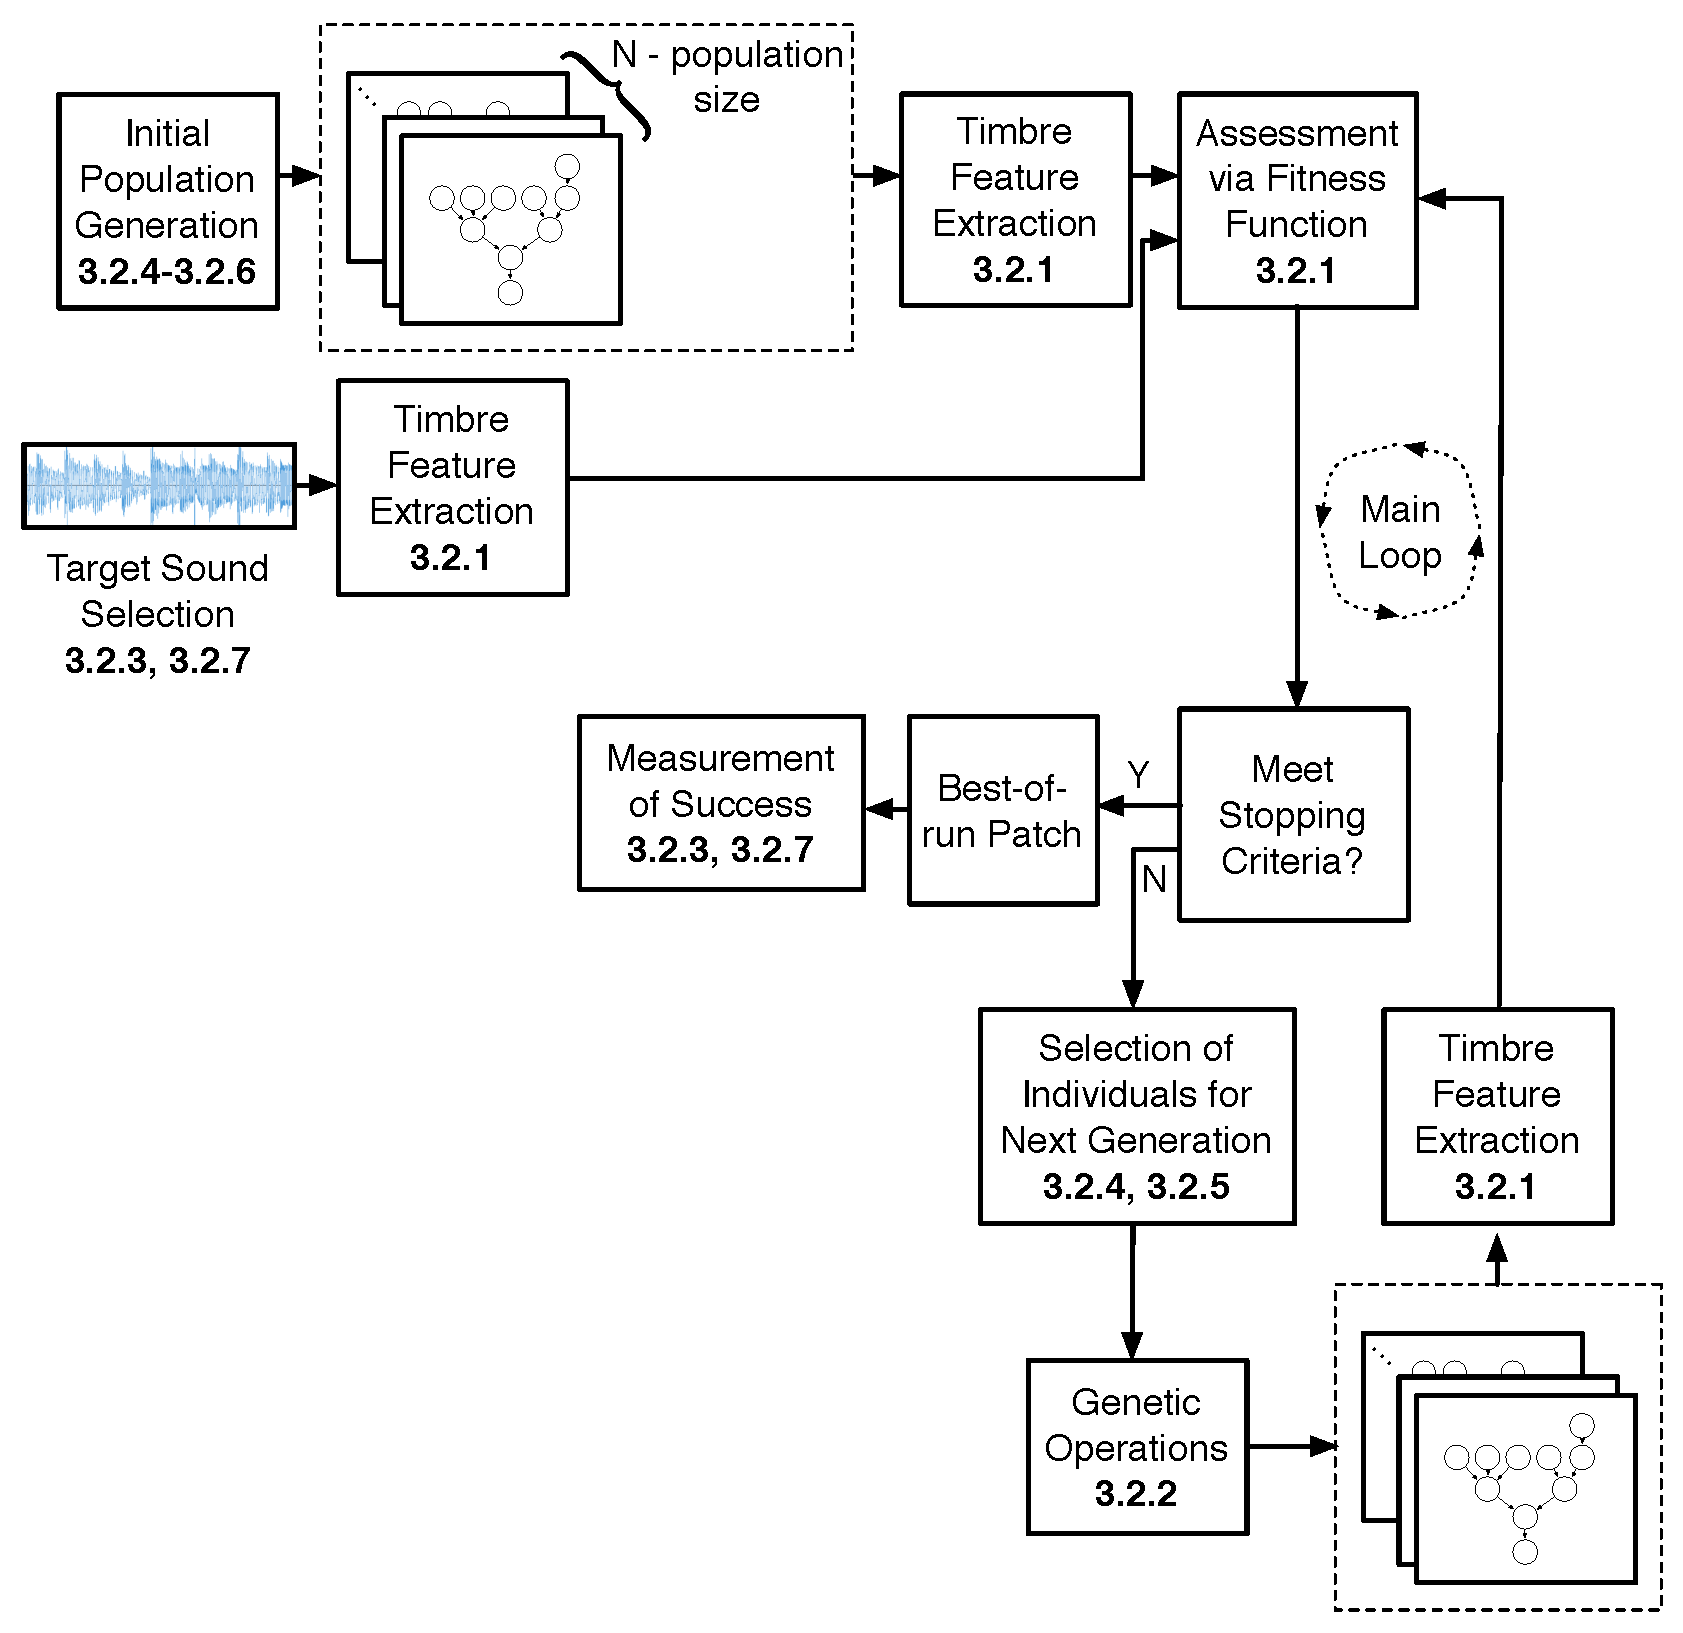
\includegraphics[scale=0.5]{OverallGPSystem}
\caption{Flow diagram of our GP system with components labeled by the section numbers they are discussed in.}
\end{center}
\end{figure}
\\
\clearpage
\subsection*{3.2 Experiment Design}
As can be seen in Figure 12, there are several modules that make up our sound synthesis search system. Each module represents at least one variable of the system that contributes to its ability to find the optimal solution as quickly (i.e. within the smallest number of iterations) as possible. Given the high-dimensionality of this variable set, it is infeasible to perform an appropriate search over all of its various permutations within a reasonable amount of time. We have chosen instead to take a measured approach to varying each variable - while holding all others constant and comparing its various values/methods using key metrics designed specifically for it - by first looking at those variables that we believe have the least amount of dependence on the settings of all others and stepping through towards those that are most dependent. Using this approach, we will be able to treat the highly dependent variables given a fixed set of near-optimal values/methods for all other variables, thereby decreasing the chance that any noticeable shortcomings of a chosen value/method for one variable are actually a result of the sub-optimal configuration of other variables that directly influence the measure we use to test it.

With this methodology in mind, we have chosen to first examine our fitness function, as it will be required to measure the success of various flavors of our system.

\subsubsection*{3.2.1 The Fitness Function}
Defining the fitness function is how one communicates to the GP system what their objective is. Without an appropriate definition, the system may discard more-optimal solutions for less-optimal ones in the eyes of the developer. This is not a shortcoming of the system itself, but instead of the developer's ability to accurately convey to the system what he is looking for. It is therefore paramount to a system's ability to produce optimal solutions to provide it with a fitness function that objectively measures the usefulness of any given solution in the same way the developer would assign value.

In this research, our objective is to generate Max patches that are able to successfully produce audio that is timbrally similar to some target sound. In order to define a fitness measure for this objective, we need to have a definition of timbre similarity. Before we can discuss an objective timbre similarity measure, we first need to have a quantitative measure of timbre. Therefore, the first task we face is choosing an appropriate timbre feature.

\subsubsection*{3.2.1.1 Timbre Feature Extraction}

The design of a semantically valid objective timbre space is paramount to the problem of search. If a timbre space has not be chosen such that meaningful timbre similarity measurements can be made, then the fitness landscape will be ill-formed and the search will pursue areas of the input space that are not relevant to the problem.

As previously discussed in the Prior Work, obtaining a ground truth to evaluate against is problematic. While most timbre space evaluation is indirectly performed via (instrument) classification tasks, due to the cost of doing large scale subjective testing, this evaluation typically assumes that all sounds produced by the same instrument have the same or similar timbre, regardless of playing technique, and so it is not clear whether or not similar evaluation methods will be valid for the �type� of timbre we are interested in. In a recent paper by Pampak, Herrera, and Goto, in referring to timbral studies that use instrument classification as a means of evaluation, the authors note that �instrument class data only allows comparison on the instrument level. Judgements within an instrument class cannot be evaluated directly� (2008, p. 9).

However, if we assume that, in general, sounds from the same instrument should cluster well in a semantically meaningful timbre space (i.e. the ratio of variance between classes/instruments should be much greater than the variance within classes/instruments), we can infer that any timbre space with that property will be organized at a high-level similarly to the optimal space. The low-level organization of the optimal space (within instrument group organization) may differ with some members of the subset of timbre spaces that have similar high-level organization and so a more rigorous treatment should be carried out to verify the appropriateness of a timbre space that organizes instrument classes well, but we leave this treatment to future work. Therefore, we assume it is enough to show that the timbre measure that we will use performs at the level of the state-of-the-art instrument recognition systems when paired with a simple classifier, like Nearest Neighbor (NN).

This relationship between classification performance and timbre space suitability provides an indirect means of testing a given timbre space. By using an unsophisticated classifier, we fully expose the organization of the space and how well instruments are clustered within it; things that could be masked by a sophisticated classifier able to overcome minor faults in both.

Nearest Neighbor classification in our case consists of mapping a large database of instrument sound samples into the objective timbre space and measuring how well they cluster by instrument by randomly choosing samples in the space, searching for their nearest neighbor in that space, and recording whether that neighbor was produced by the same instrument. One is then able to compare multiple objective spaces by using the �classification� accuracy found during the experiment. This method is often extended to reduce noise by selecting k-nearest neighbors (kNN) and noting how many of the k neighbors were produced by the same instrument as the test sample (see Figure 14).
\begin{figure}[h!]
\begin{center}
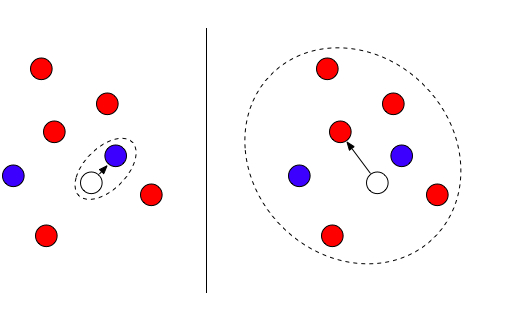
\includegraphics[scale=0.5]{NearestNeighbor}
\caption[Nearest-neighbor vs. k-nearest neighbor classifier]{Nearest-neighbor vs. k-nearest neighbor classifier - the test sample (white) is set to the blue class in nearest-neighbor classification and to the red in k-nearest neighbor classification where k = 7}
\end{center}
\end{figure}
\\
Given the above, we have decided to measure the appropriateness of a given objective timbre space by running an instrument classification experiment on it using a kNN classifier.

In a paper we have helped author (Humphrey, Glennon, and Bello, 2011) we discuss our belief that it is `advantageous to automatically learn features from some minimally processed input representation' rather than hand-craft a feature set that would produce a semantically meaningful timbre space. In short, learning features allows one to explicitly specify how they want a feature-space organized (in our case, well-clustered instrument samples) and leverage machine learning algorithms to find an optimal space for that criteria, whereas designing features based either on perceptual models or what one believes to be the important information content related to a task is just a guessing game with no proven iterative search strategy, likely excluding optimal solutions simply because they are non-intuitive or obfuscated from the researcher in some way.

The technique that we have helped develop to learn an appropriate timbre space where different instruments are well-clustered is titled `Non-linear Semantic Embedding (NLSE).' In our paper we note:
\begin{quote}
NLSE addresses the limitations of current statistical dimensionality reduction techniques, such as MDS, PCA or LLE [because] unlike these methods, NLSE explicitly encodes semantic information in the transformation, makes minimal assumptions about salient acoustic features, generalizes well to unseen data and produces an output space where [Euclidean] distance is meaningful.
\end{quote}

NLSE utilizes a pairwise Convolutional Neural Net (CNN) model based upon Hadsell, Chopra, and LeCun's work on Dimensionality Reduction by Learning an Invariant Mapping (DrLIM) (2006). CNNs are a special kind of Neural Net that combines convolutional layers (where inputs are convolved with 2D filters, whose values are trainable) that are typically separated by a downsampling operation and a non-linear squashing function (see Figure 14). After a succession of these convolution layers, CNNs most often use standard fully-connected NN layers to reduce the dimensionality of the data before output. The benefits of CNNs are found in the translation invariance their convolutional layers provide, and scale invariance the downsampling operation provides. When the input to a CNN is a time-frequency representation as is the case in our problem domain, these invariances correspond to small invariances in temporal shifts and scalings in our data (important because we should not suppose that all samples will be precisely temporally aligned or that their timbral information will evolve precisely in the same manner) and small invariances over our frequency scale. The latter invariance is important to extracting timbre from a signal, because it is generally believed that timbre does not correlate with pitch variation. It is therefore possible to utilize the inherent frequency scale invariance that CNNs provide to better eliminate any dependencies in our output space on pitch by using a time-frequency representation that is linear in pitch. For this reason, we have chosen a constant-Q time frequency representation as is shown in Figure 14, where bins are spaced equally in pitch space rather than in frequency space.

Hadsell, Chopra, and LeCun's work on DrLIM utilizes a pairwise CNN architecture (ie. two CNNs with the same exact structure) with tied weights to learn a low-dimensional invariant mapping from a high-dimensional input space. The training phase consists of sending both positive (i.e. samples from the same instrument) and negative (samples from two different instruments) examples through the CNNs and adjusting the tied weights such that semantically similar items are placed near each other in the output space and semantically dissimilar items are placed far away from each other in the output space. This is accomplished using what is known as a `contrastive loss function.' The basic idea is that one establishes a loss function that returns small values for positive examples that are close to one another in the output space and large values for positive examples that are far away from one another in the output space and conversely returns small values for negative examples that are far away from each other in the output space and large values for negative examples that are close to each other in the output space. Specifically, the loss function we have chosen that meets this criteria follows:
\begin{equation}
L(X_1, X_2, Y|W)=Y*L_{sim}(D)+(1-Y)*L_{Diff}
\end{equation}
The inputs $X_1$ and $X_2$ to L represent our constant-Q time-frequency patches, Y is our semantic similarity score between our inputs taking a value $[0,1]$ and W represents the parameters of the CNN architecture. $L_{Sim}(D)$ and $L_{Diff}(D)$ are our similarity loss and difference loss, respectively and D is some cost function associated with the outputs of our architecture, often labeled $Z_1$ and $Z_2$. In our system, this cost function is simply the Euclidean distance between the points $Z_1$ and $Z_2$.

Note that the only contributor to our contrastive loss, L, is the similarity loss when $Y=1$ (i.e. the items are maximally similar) and the only contributor to L is the difference loss when $Y=0$ (i.e. the items are maximally dissimilar). Since we want the loss to increase for similar items that are far apart, we chose the following similarity loss (known as the square loss):
\begin{equation}
L_{Sim}=\frac{1}{2}Y*D^2
\end{equation}
Note that as the distance between points increases, so does the loss. Conversely, we want the difference loss (which contributes most when items are maximally dissimilar) to increase as the distance between $Z_1$ and $Z_2$ decreases. We therefore chose the following difference loss (known as the `log-loss'):
\begin{equation}
L_{Diff}=\frac{1}{2*Q^2}*log\Big(1.0+e^{Q*(m-D)}\Big)^2
\end{equation}
The parameters $m$ and $Q$ are used to define the loss function's `margin' and `knee' respectively, but the details of this are not important. The important thing to note is that as $D$ decreases, $e^{Q*(m-D)}$ increases, which in turn increases $L_{Diff}$ as desired.

By using standard back propagation methods, one is able to update all the trainable parameters in the CNN architecture so that, over $N$ iterations, the parameters converge to a stable state (and hopefully a global optimum). Once convergence occurs, the resulting pairwise architecture represents two copies of a CNN that has learned a low-dimensional invariant mapping from the high-dimensional input space of your original data (e.g. patches of constant-Q spectra) into a semantically meaningful low-dimensional space. In our problem domain, this means a timbre space where samples from the same instrument class are well clustered and instrument clusters are well-separated.
\begin{figure}[h!]
\begin{center}
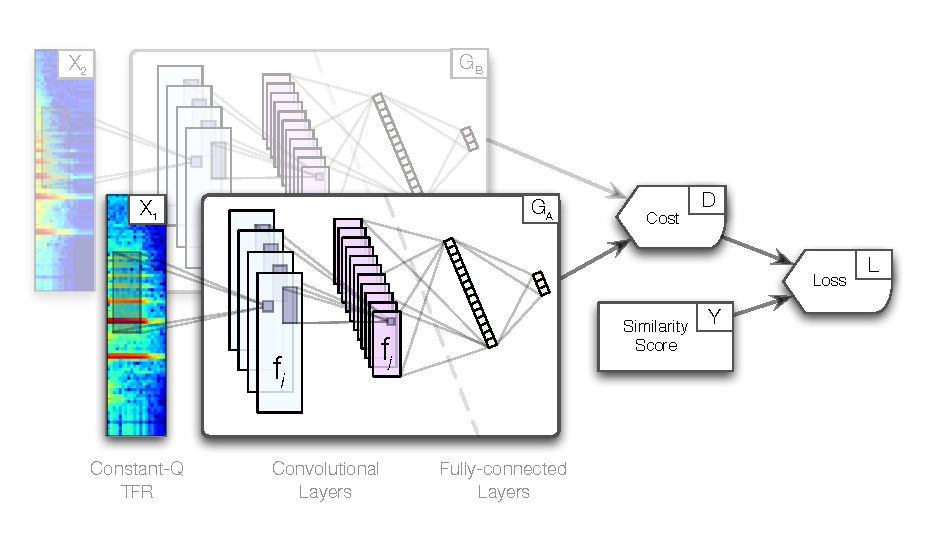
\includegraphics[scale=0.95]{PairwiseCNN}
\caption[Pairwise CNN Architecture]{Pairwise CNN used to learn an objective timbre space from various pairs of within class and between class instrument samples.}
\end{center}
\end{figure}
\\
As is shown in our paper, the objective timbre space we have generated (and the corresponding features that define the space) outperform the leading alternative timbre-feature in the literature (MFCCs) - after the typical PCA and LLE dimensionality reduction techniques have been applied - on instrument classification tasks involving up to 12 different instruments (see Figure 15 for kNN accuracy up to 9 instruments). Specifically, NLSE remains at a classification accuracy above 90\% until 7 instruments are introduced, while PCA and LLE are both between 30\%-40\% lower than NLSE for all cases.
\begin{figure}[h!]
\begin{center}
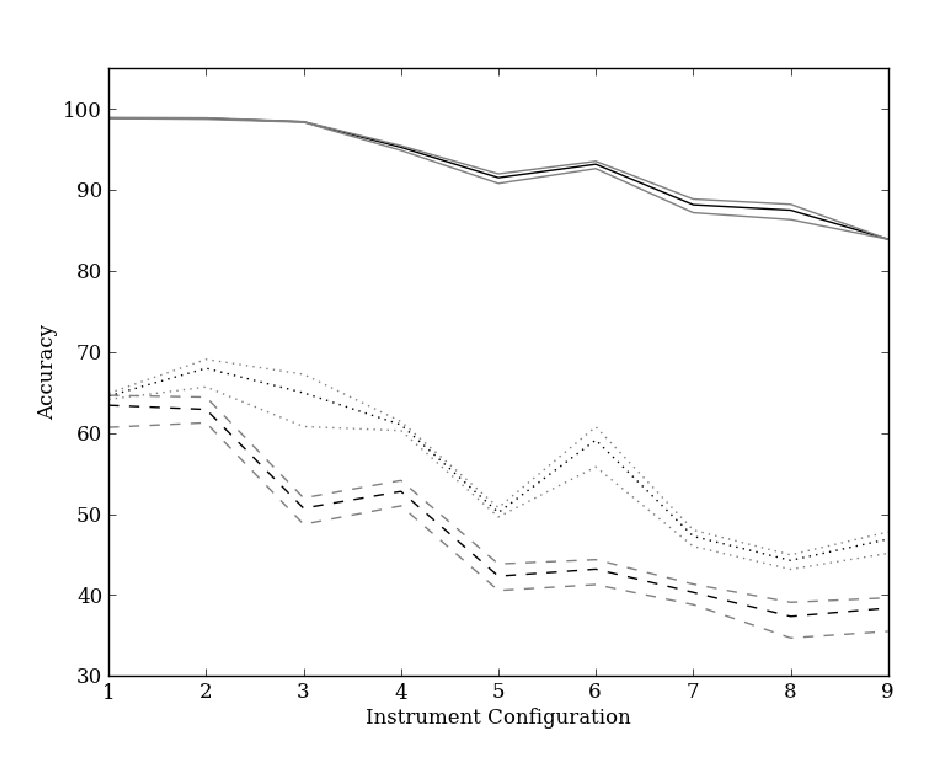
\includegraphics[scale=0.85]{CNN_kNN}
\caption[kNN accuracy for NLSE, PCA, and LLE]{The mean, min, and max kNN accuracy for experiments varying k using NLSE (solid lines), PCA (dotted lines), and LLE (dashed lines).}
\end{center}
\end{figure}
\\
For some intuition on how the objective timbre output spaces are organized in the NLSE, PCA of MFCC, and LLE of MFCC cases, see Figure 16 showing the distribution of instrument samples for 5 different instruments.
\begin{figure}[h!]
\begin{center}
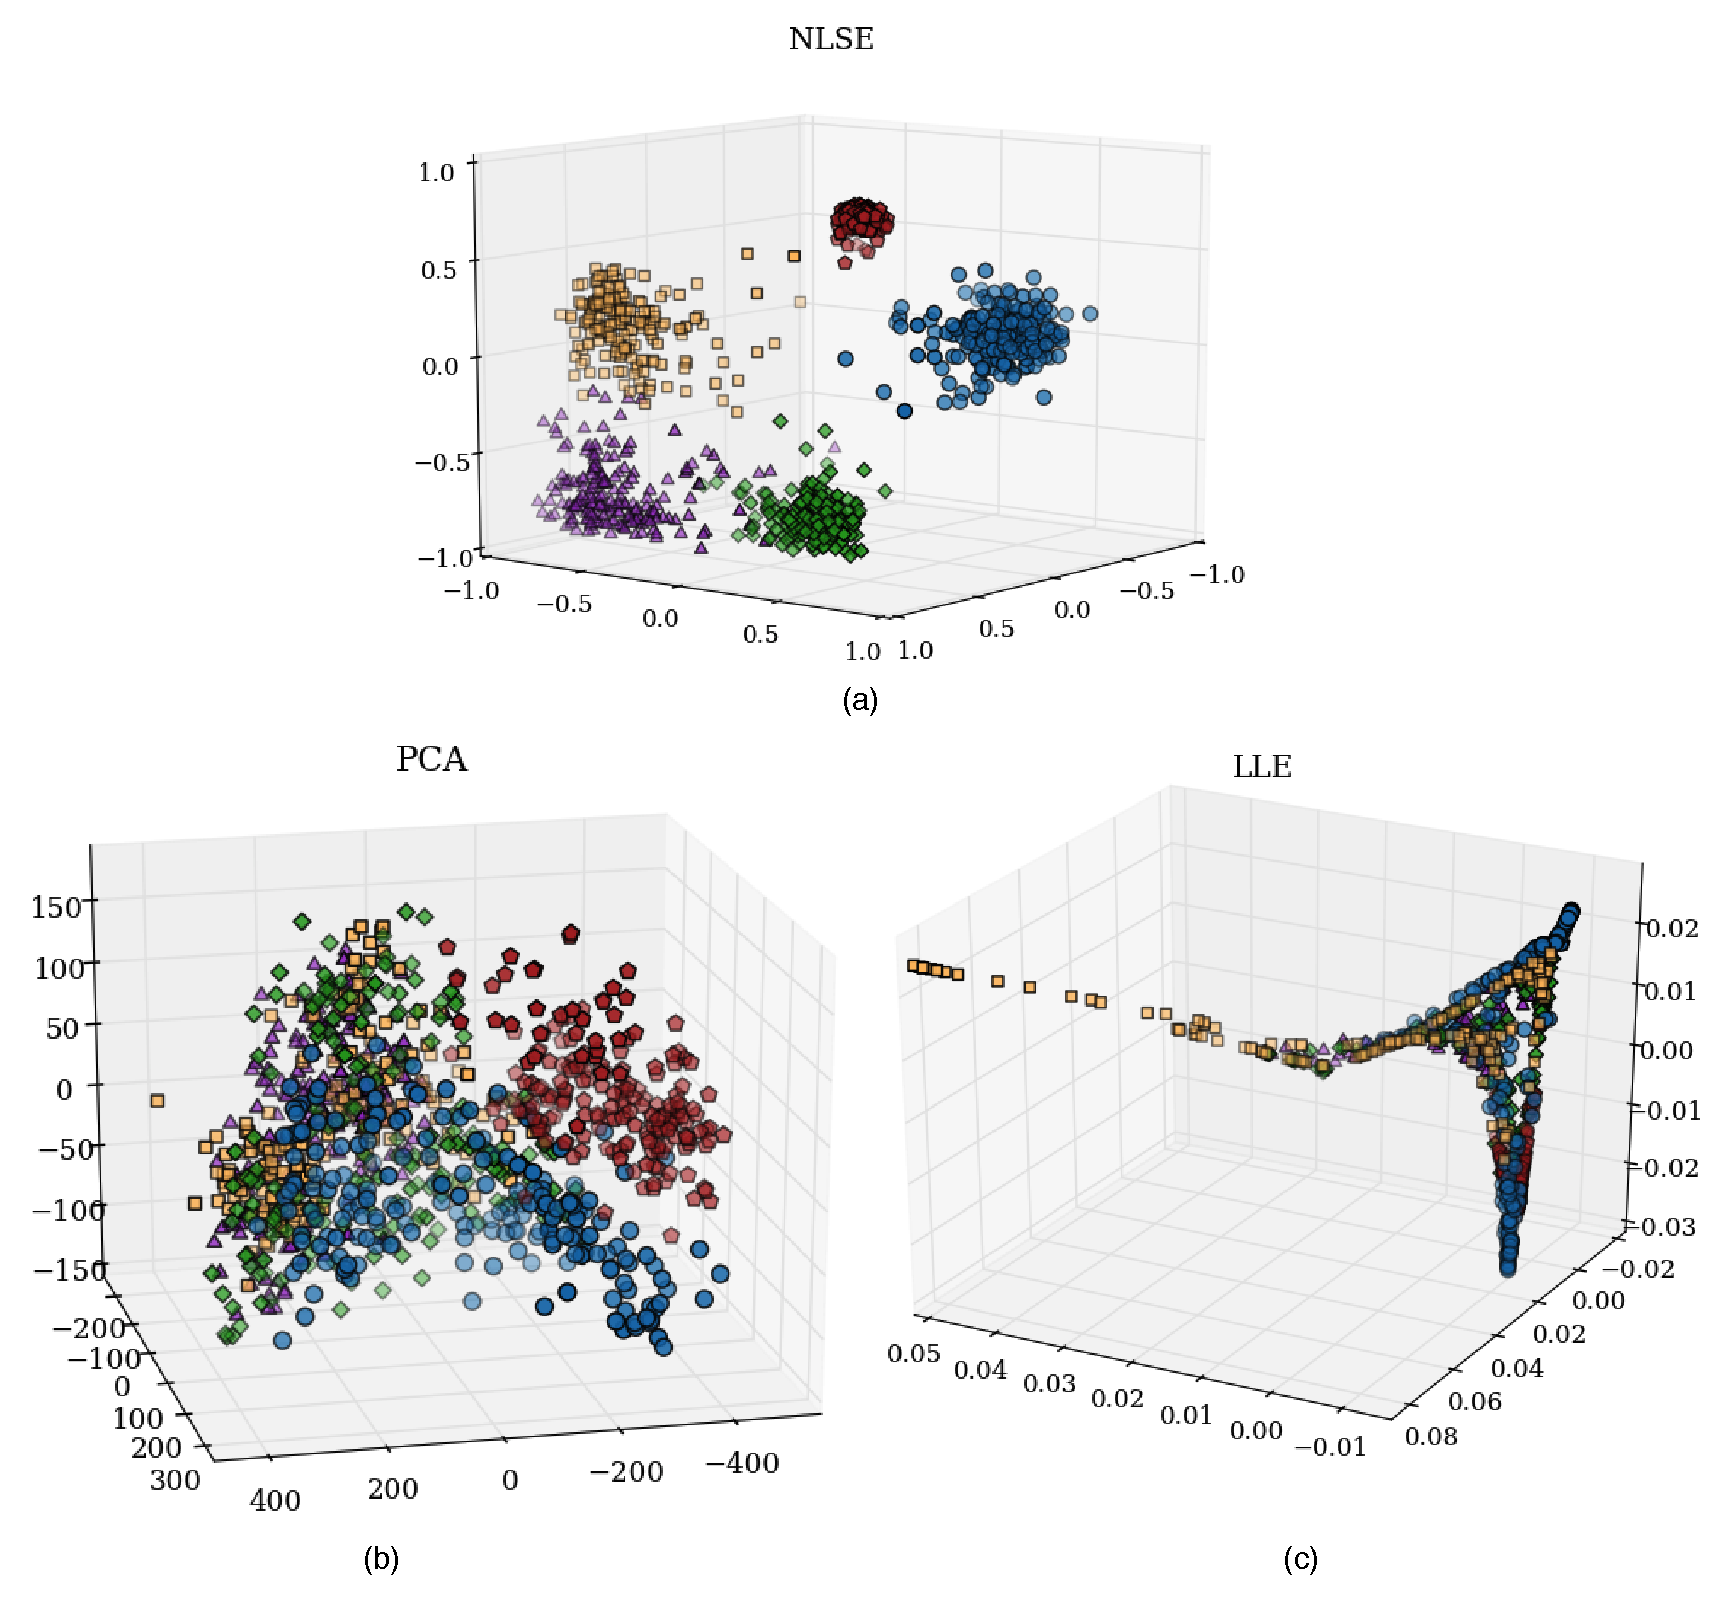
\includegraphics[scale=0.55]{NLSECluster}
\caption[NLSE vs. PCA vs. LLE Instrument Clusters]{Output feature spaces generated by (a) NLSE, (b) PCA, and (c) LLE for Tuba (red pentagons), Oboe (green diamonds), Clarinet (purple triangles), Cello (blue circles), and Flute (yellow squares).}
\end{center}
\end{figure}
\\
\subsubsection*{3.2.1.2 Timbre Similarity}

Given the timbre features we have developed using CNNs, we must develop a measure of timbre similarity for time-varying timbres in the space our features define. Timbres that do not vary over $N$ time-frequency patches will only occupy a small region or point in this space. The calculation of timbre similarity between static or near-static timbres of this sort can simply be approximated using the Euclidean distance between the individual distribution centers since the space is trained for this distance to be semantically meaningful (see Figure 17). 
\begin{figure}[h!]
\begin{center}
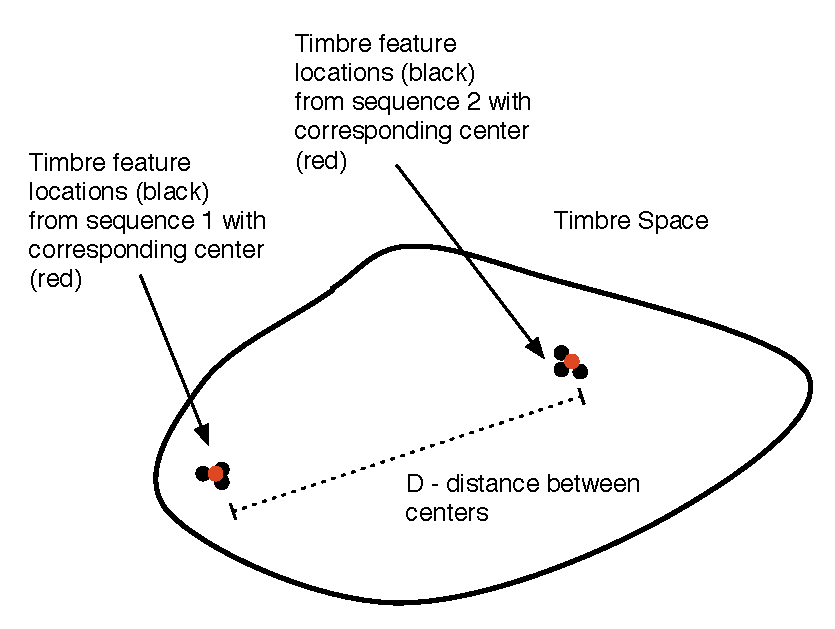
\includegraphics[scale=0.8]{TimbreDistance1}
\caption[Timbre Distance Between Centers]{Timbre similarity between two sequences of time-frequency patches approximated using the distance between their centers.}
\end{center}
\end{figure}
\\
However, the calculation of timbre similarity becomes more complicated once a sound contains timbal variation corresponding to a traced out path in timbre space away from the region in which it started. The task then becomes measuring similarity between two traced out paths in timbre space (see Figure 18). 
\begin{figure}[h!]
\begin{center}
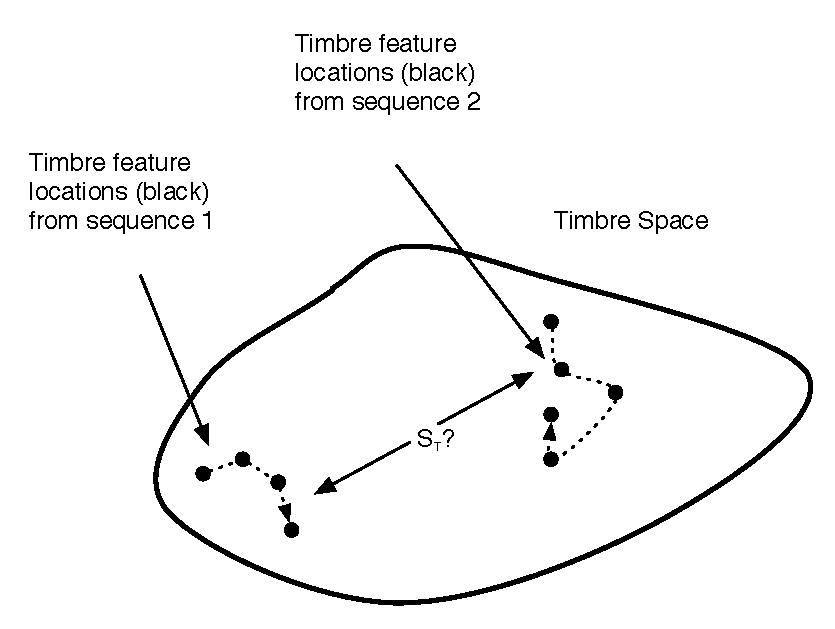
\includegraphics[scale=0.8]{TimbreDistance2}
\caption[Timbre Distance Between Curves]{How does one calculate the similarity or distance between two curves in timbre space that are not well localized?}
\end{center}
\end{figure}
\\
Since points in timbre space will occur at regular discrete intervals in time, the paths actually represent discrete sequences of timbre points. Therefore, the question we must answer is "How should one measure the timbre similarity between two discrete sequences (possibly having different lengths) of timbre feature vectors?" If we only allowed comparisons between sequences of equal length, a common solution would be to line up points in the two feature vector sequences, calculate the Euclidean distance between the pairs of lined up points, sum all distances, and take the inverse of the result (referred to as the `aligned-Euclidean' method going forward):
\begin{equation}
S_T = \sum_{i=1}^{M}\sqrt{\sum_{j=1}^{N}(Z_{ij}^1 - Z_{ij}^2)^2}
\end{equation}
where $Z^1$ and $Z^2$ represent the two sequences of timbre feature vectors (obtained via processing of time-frequency patches through our trained CNN architecture) to compare, N is the dimensionality of the timbre feature space, and M is the length of each sequence.

However, even given the restriction of equal sequence lengths (which is obviously undesirable) there are many examples where this measure will break down. For example, if one takes two copies of the same exact sound and applies a simple linear time shift to one (i.e. a delay), the suggested similarity calculation could result in labeling the two sounds as being very distant (see Figure 19).
\begin{figure}[h!]
\begin{center}
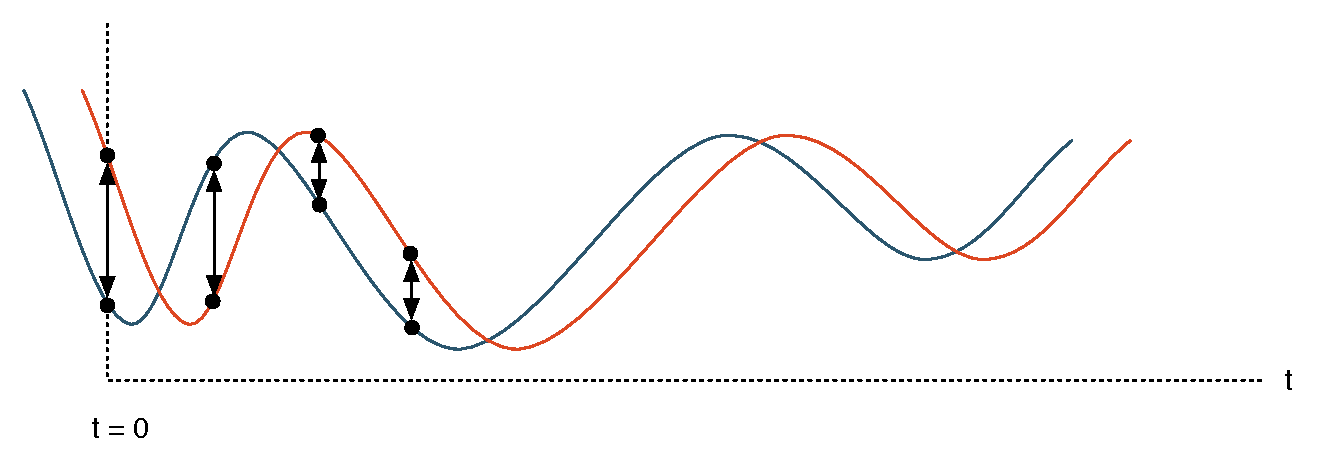
\includegraphics[scale=0.6]{TimbreDistance3}
\caption[Timbre Distance Between Time-Shifted Curves]{An example of how a simple temporal shift of the exact same curve can result in non-negligible distance calculations between corresponding points in the resultant discrete sequences.}
\end{center}
\end{figure}
\\
Slight time warpings of one sound compared to the other would also result in an incorrect assessment (see Figure 20). It is for this reason that Jehan uses Dynamic Time Warping (DTW) when calculating similarity over sound segments (2005). The only difference between the problem he was addressing and ours is the time scale on which similarity is being computed. 
\begin{figure}[h!]
\begin{center}
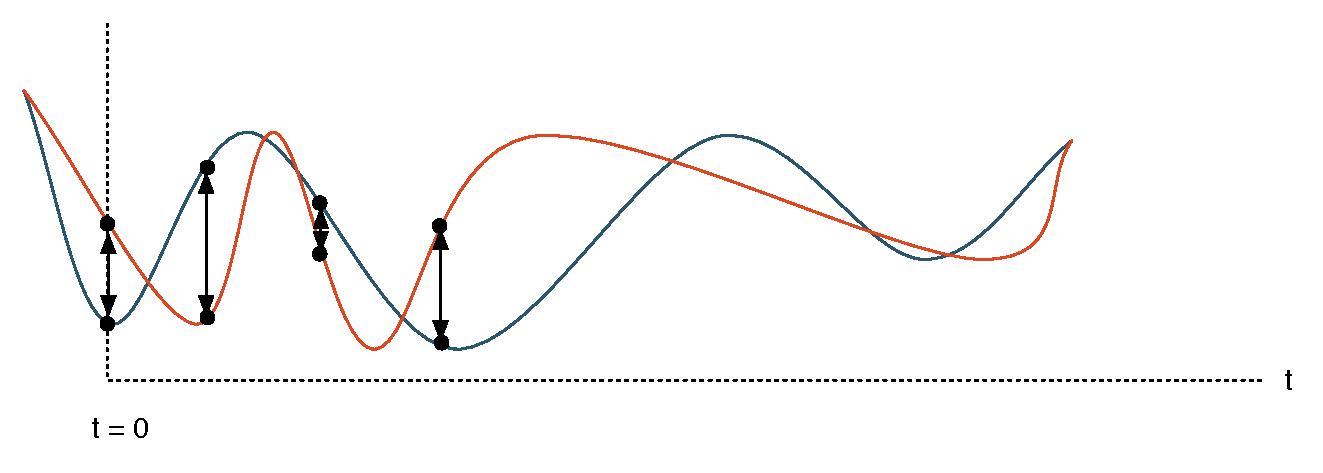
\includegraphics[scale=0.6]{TimbreDistance4}
\caption[Timbre Distance Between Time-Warped Curves]{An example of how a temporal warping of the exact same curve can result in non-negligible distance calculations between corresponding points in the resultant discrete sequences.}
\end{center}
\end{figure}
\\
DTW is a sequence similarity calculation method that attempts to align the time scales over which two different sequences of data occur by finding the optimal warping path between those time scales before calculating the distance over pairs of aligned points in the two sequences. For a more detailed overview and a real-time implementation of a close approximation, see (Salvador and Chan, 2004). We provide a diagram of the best warping path given the two sequences found in the previous figure in Figure 21. 
\begin{figure}[h!]
\begin{center}
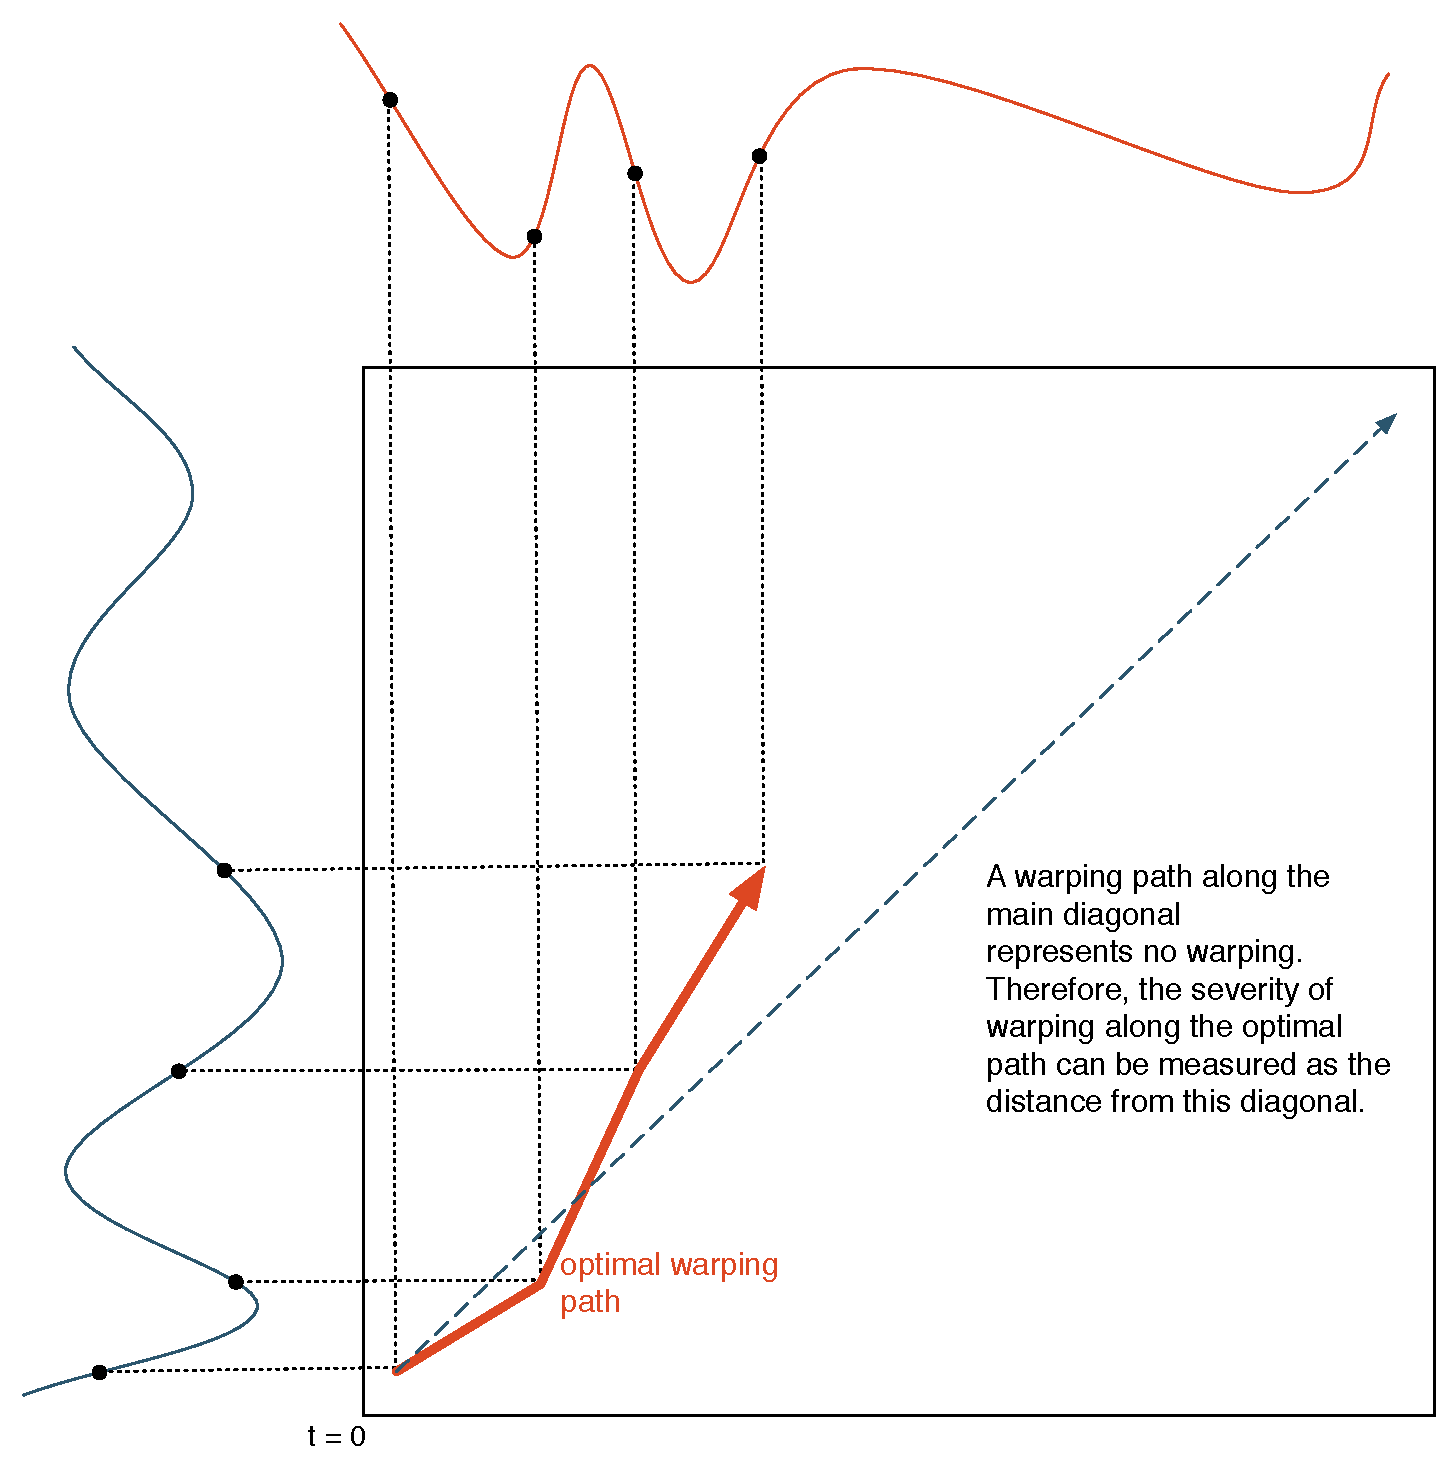
\includegraphics[scale=0.5]{DTWExample}
\caption[Timbre Distance Between Time-Warped Curves]{The optimal warping path between the two sequences from Figure 20 is shown.}
\end{center}
\end{figure}
\\
Note that given the optimal warping path, the sequences look identical (exemplified by the aligned points in the figure). Given the alignment this produces, accumulating distances between aligned pairs would result in a very small sequence distance and therefore a very high similarity.

DTW can be performed on sequences that have different lengths, which obviates the need for the same-length restriction required for the aligned-Euclidean measure. It is also important to note that if two timbre sequences are not time shifted or time warped, but instead could accurately be described using the aligned-Euclidean distance measure, DTW will most-often return a warping path that is near linear (i.e. very close to the main diagonal) so that the DTW result will match the aligned-Euclidean result. For this reason, the DTW measure can be seen as a more robust version of the aligned-Euclidean measure.

While DTW provides a metric that is invariant to time shifts and warpings and other temporal distortions (e.g. random sample deletion and random extension of static timbal content), there are situations in which it is not sufficient. The major drawback of DTW is that it requires that the beginning and ending of each sequence is aligned and that both sequences move forward in time from beginning to end. In other words, it can only search for the best global warping between two sequences. This is problematic given two sequences that are produced by the same object, but that contain a different amount of similar repeated subsequences. An example in our problem domain would be if we had two audio clips of the same bird chirping and breathing (labelled $A$ and $B$, respectively), with one clip containing three chirps followed by one breath ($AAAB$) and the other containing two chirps followed by one breath, followed by another two chirps ($AABAAB$). DTW would only search for paths that would align the two global sequences (likely resulting in a linear path through the first two $AA$s in each sequence and then stumbling to find an appropriate match to the third $A$ in the first sequence) and would fail to find an appropriate path to consider these two sequences similar, even though they in fact contain timbal subsequences that are almost exactly the same and that follow a similar sequencing of several $A$s followed by a $B$ (Serr\`a, G\'omen, Herrera, and Serra, 2008, p. 1143).

One solution is to eliminate the global alignment requirement of DTW. Serr\`a et al. propose a method they call Dynamic Programming Local Alignment (DPLA) that leverages both principles of DTW and the Smith-Waterman algorithm (a technique used in molecular biology that compares subsequences of all possible lengths to optimize a similarity measure) to find the longest similar subsequences from two sequences. DPLA uses only the data from those most-similar subsequences to calculate a similarity measure for purposes of cover song identification. In their problem domain, this measure works well because it is completely natural for cover songs to contain segments that are wholly different from the original and which therefore should be ignored as long as there is a long enough segment/subsequence that matches well with the original. In other words, an original song with structure $ABABC$ may have a cover with structure $BAADE$ (In this example, letters refer to subsequences of time-frequency patches that may or may not repeat within the overall sequence). Given the common occurence of such dramatic structural changes, these sequences should be considered similar and DPLA labels them as such. This is not an optimal similarity measure for timbre however, as a brief moment of a similar texture surrounded by vastly different sonic textures should not be considered to have an overall similar timbre evolution. While we do not want to enforce a global warping when comparing two timbre sequences, we do want a measure that takes the global sequences into account.

Given this, our approach extends DPLA to look for the best sequence of local subsequence alignments, where subsequences may be repeated, internally warped, and placed out of order, but such transformations are penalized. We have decided to penalize these transformations because we believe that too much of any will disrupt the overall sense of timbre. For example, a sequence of $ABCABC$ will be considered more similar to $AABCABC$ than $AAAABCABC$, more similar to $ABCABC$ where all subsequences are of the same length to those in the original $ABCABC$ than an $ABCABC$ where they are not, and more similar to $ABCABC$ than $CBABAC$.

An initial approach given the above could use a greedy algorithm that utilizes DPLA to find the longest common subsequence between sequences, removes those subsequences and repeats the process until an appropriate stopping criteria is met (e.g. the remaining sequence length after removing all paired subsequences is less than some threshold). However, the problem with this approach is that in certain cases a removed subsequence, $A$, may in fact be composed of two smaller subsequences, $B$ and $C$, one of which is repeated several times in one sequence and only once in the other. By removing $A$, $B$ and $C$ are also removed and therefore a repetition of $B$, for example, in one sequence would have no matching $B$ in the example with its only instance held within $A$ (see Figure 22).
\begin{figure}[h!]
\begin{center}
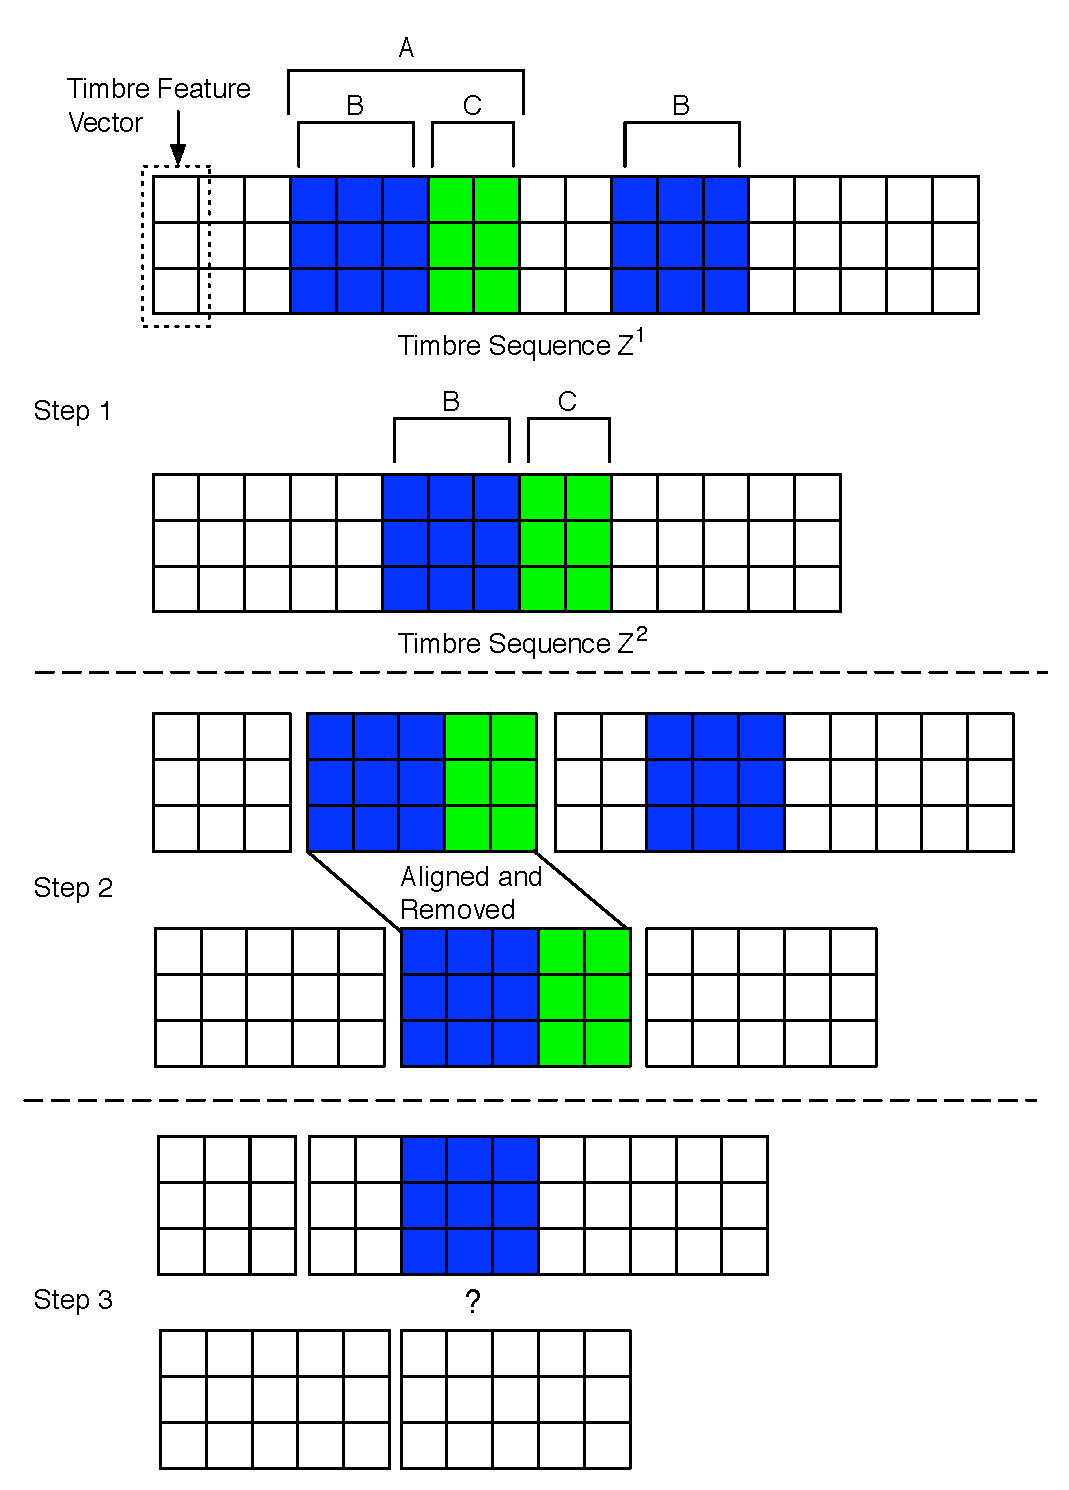
\includegraphics[scale=0.6]{GreedyMatching1}
\caption[Symmetric Greedy Removal After Matching]{In step 1, we search for the optimal local alignment between the two sequences. Once we find that alignment in step 2, we remove the subsequences involved from further consideration. In step 3, we have left a repetition of subsequence B stranded without a corresponding match in the second sequence.}
\end{center}
\end{figure}
\\
This issue arises because of the greediness of the approach. By removing a subsequence from contention from one sequence that the other could re-use to find an appropriate alignment to another one of its subsequences (e.g. $B$ in this example), we have weakened our ability to fairly find the best combination of optimal local alignments. We have given preferential treatment to one sequence (that which does not require an aligned repetition of $B$) over the other. This situation can occur over a single set of two sequences in both directions, so it isn't a matter of determining which sequence to prefer in our search if we use this greedy approach. 

A slightly less greedy option is to only eliminate the aligned subsequences of one sequence while allowing re-use of the entire other sequence throughout the alignment process. In other words, we start by finding the best subsequence alignment between two sequences $Z^1$ (the superior) and $Z^2$ (the inferior), remove that subsequence from $Z^1$ (but not from $Z^2$) and then search for the best local alignment between the two left over pieces of $Z^1$ and the entirety of $Z^2$, continuing along until all of $Z^1$ is aligned to some part of $Z^2$ (see Figure 23). 
\begin{figure}[h!]
\begin{center}
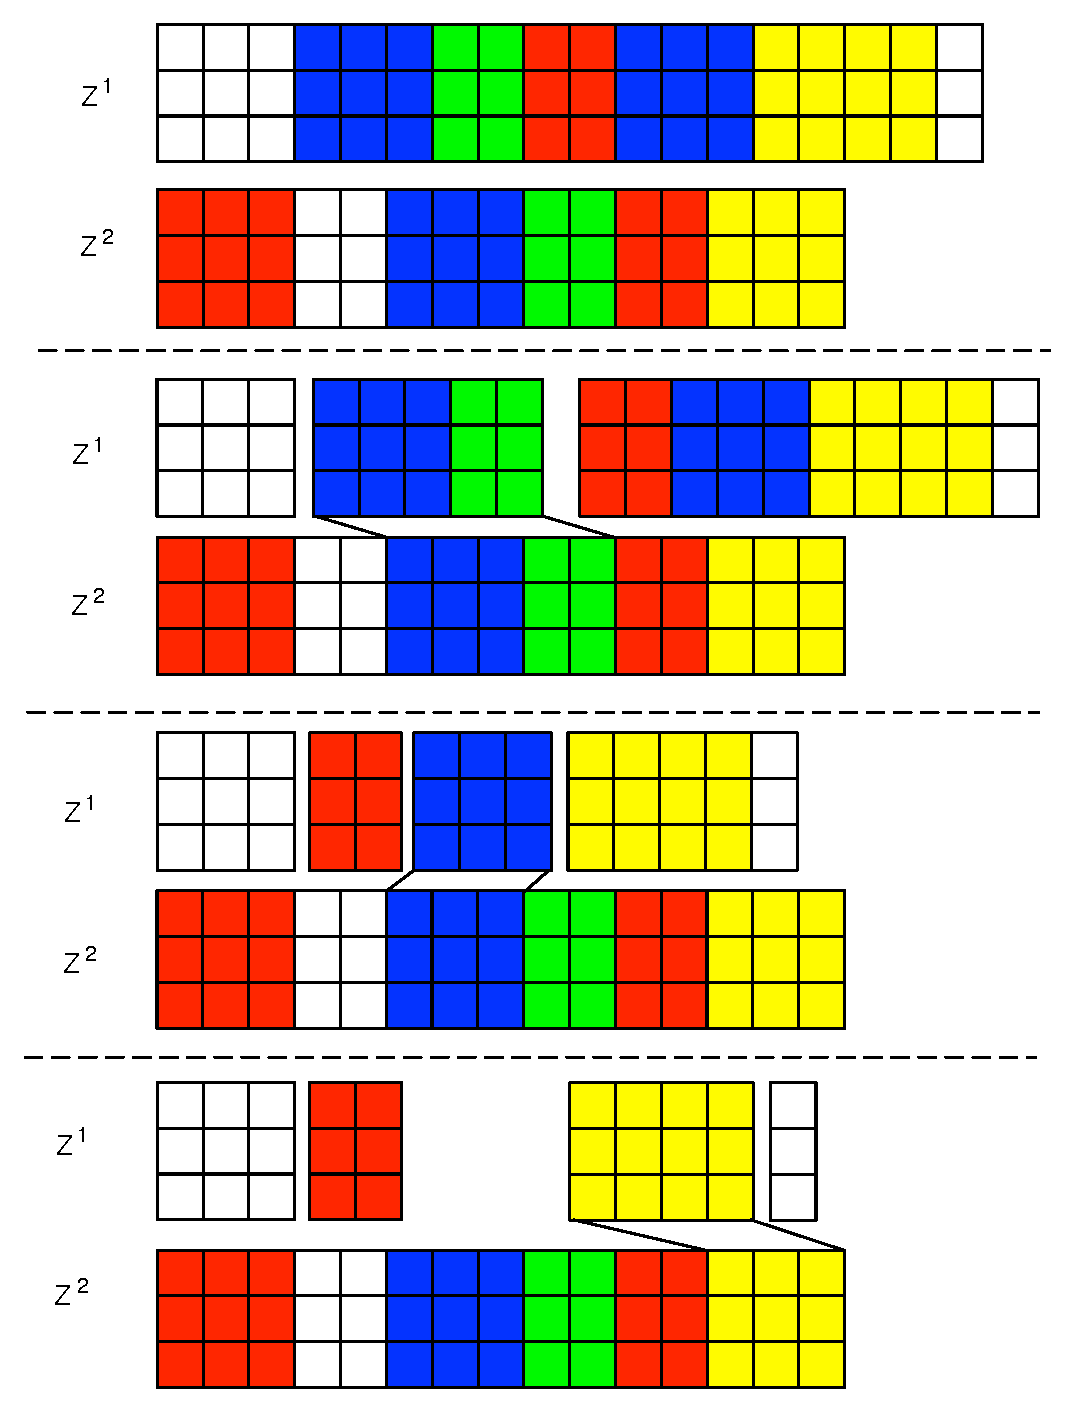
\includegraphics[scale=0.65]{GreedyMatching2}
\caption[Asymmetric Greedy Removal After Matching]{The optimally matched subsequences of $Z^1$ are removed after they are found, while $Z^2$ remains intact to provide $Z^1$ with the ability to match numerous subsequences to the overlapping content in $Z^2$}
\end{center}
\end{figure}
\\
This method obviously is biased towards finding appropriate matches in $Z^2$ to all of $Z^1$ (and not vice versa), but can be made symmetric by repeating the process in the opposite direction (removing aligned subsequences of $Z^2$ along the way, but reusing any aligned segments of $Z^1$) (see Figure 24). 
\begin{figure}[h!]
\begin{center}
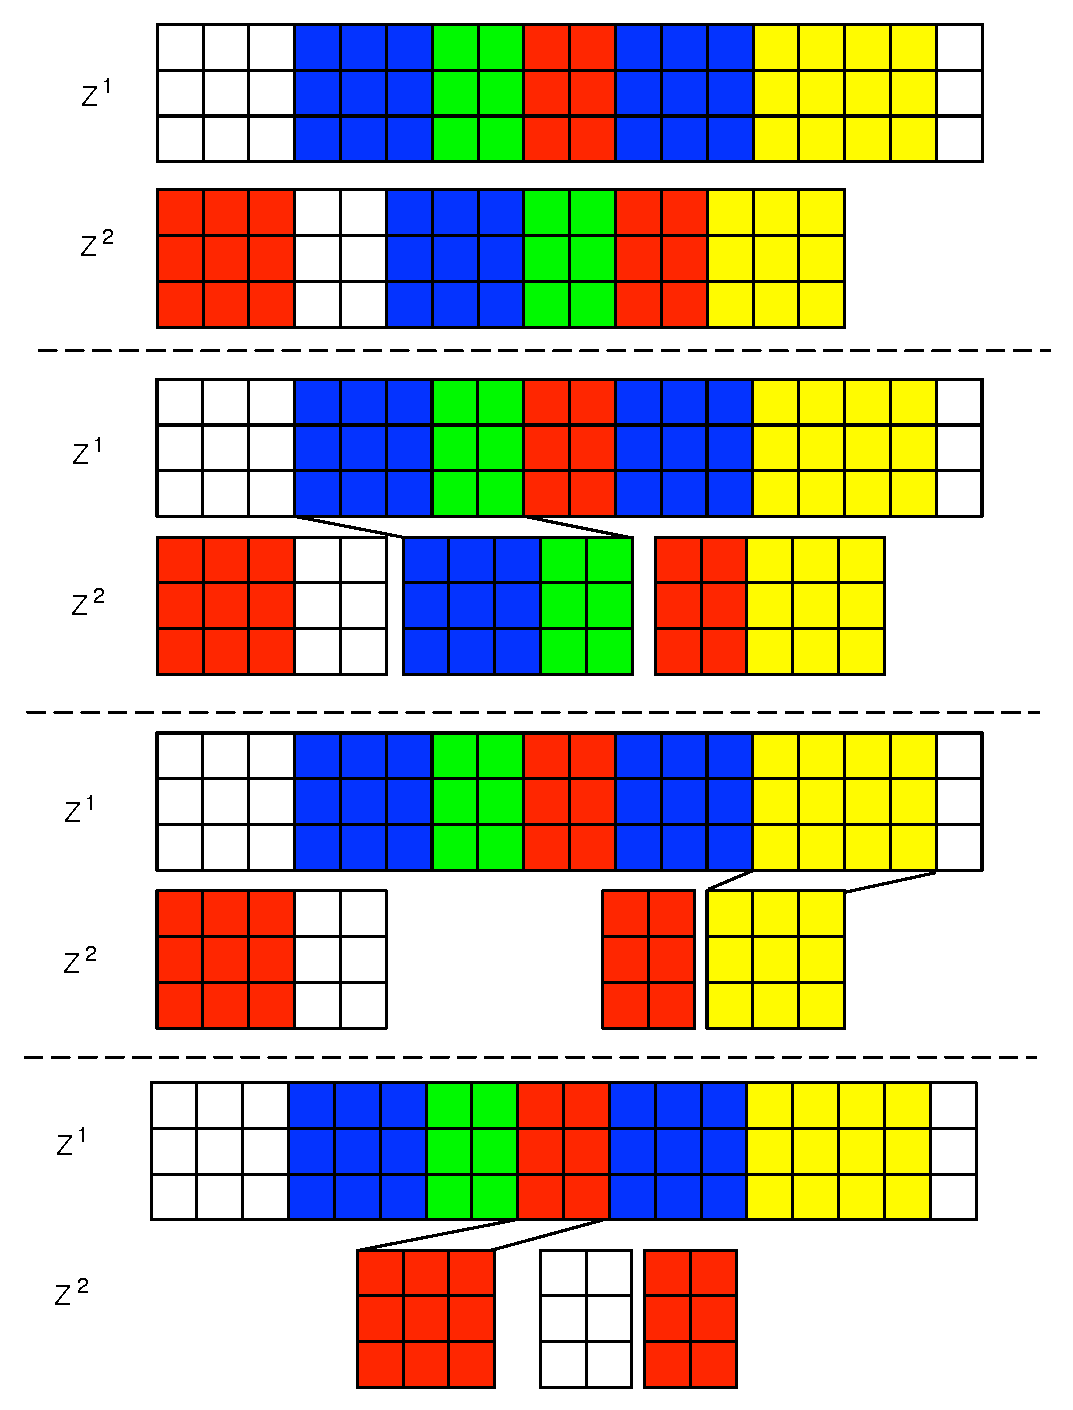
\includegraphics[scale=0.65]{GreedyMatching3}
\caption[Asymmetric Greedy Removal After Matching Reverse]{The optimally matched subsequences of $Z^2$ are removed after they are found, while $Z^1$ remains intact to provide $Z^2$ with the ability to match numerous subsequences to the overlapping content in $Z^1$}
\end{center}
\end{figure}
\\
The alignment combinations that are produced for each process can be used to calculate individual distance scores and then summed for a symmetric measure of similarity between both sequences:
\begin{equation}
S_T = \frac{2}{D_{SICSW}} \equiv \frac{2}{D_{ICSW_{1\to2}} + D_{ICSW_{2\to1}}}
\end{equation}
where $D_{SICSW}$ is what we call the Symmetric Iterative Continuous Smith-Waterman (SI-CSW) distance, $D_{ICSW_{1\to2}}$ is what we will call Iterative-CSW (I-CSW) distance calculated when treating $Z^1$ as the superior sequence (defined below) and $D_{ICSW_{2\to1}}$ is the I-CSW distance calculated when treating $Z^2$ as the superior sequence.

The remaining question is how one calculates the SI-CSW distance based on a number of subsequence alignments that may or may not be ordered appropriately in time, may or may not overlap in one or both sequences (this including repetitions), and may or may not include the entirety of both sequences. All of these must be considered in determining an asymmetric global sequence similarity score before averaging this measure over the results of the process in both directions. To begin, we must briefly overview the Smith-Waterman algorithm and discuss how we can leverage it for our problem domain.

As previously mentioned, DPLA utilizes the Smith-Waterman technique for performing local sequence alignment. This technique was first discussed towards finding ``maximally homogenous subsequences among sets of long sequences...in molecular sequence analysis.'' This problem domain differs from ours (as well as that of Serr\'a et al.) in that molecular sequences contain a fixed set of discrete values. This is an important distinction, because the Smith-Waterman technique typically is used in a problem domain where one will often find exact subsequence matches within a sequence. In its basic form, it takes a binary similarity matrix as its input based on this assumption, where one of the possible values represents `sameness' and the other, `difference.'

The way the Serr\'a et al. generate a binary similarity matrix between Harmonic Pitch Class Profile (HPCP) vectors - a standard, continuous-valued feature in the domain of cover song identification - is by using a thresholded similarity function with binary output (2008). If two HPCP vectors are similar enough, this threshold function considers them the same and if they are not, different. Serr\'a et al.'s ability to transform their problem into one that looks typical for Smith-Waterman allows them to use the technique `out of the box.' However, the goal of most problems utilizing the Smith-Waterman algorithm is slightly different from ours (in that we do not only consider exact matches between timbre vectors as being similar) and therefore we have decided not to try to transform our problem into one its standard implementation understands, but instead we have chosen to transform its standard implementation to one that fits our problem.

The Smith-Waterman algorithm assigns a positive value to two similar vectors and a negative value to two dissimilar vectors, so that ``these values have an average for long, random sequences...of zero.'' (Smith and Waterman, 1981, p. 196). This is important because we will be looking at the cumulative sum of these values over subsequences of vectors to determine whether they align well. If the cumulative sum is greater than $0$, we can assume this is not by chance and that these two subsequences should be aligned. In the standard implementation, pairs of vectors can only be labelled `similar' or `dissimilar' and therefore will only take on either a single positive value or a single negative value. By comparing all pairs of vectors in two sequences this way, one obtains a binary similarity matrix, $S$, where its elements $s_{ij}$ are positive if vector i from the first sequence and j from the second sequence are similar and a negative value if they are dissimilar.

However, the standard calculation of a binary similarity matrix is not required for Smith-Waterman to function appropriately. The important part of Smith-Waterman - and that which separates it from something like DTW - is that it creates inherent segmentation boundaries for optimally aligned subsequences due to its summation of both positive and negative similarity values. As already stated, the technique looks for subsequences who, over their length, accumulate positive similarity values (as will be discussed in detail below). Once these accumulations start to trend negatively, the alignments can be considered complete and local subsequence alignment boundaries are defined. Therefore, continuous valued similarity matrices may be used in Smith-Waterman as long as the elements can take both positive and negative values.

In our problem domain, we have already defined a similarity measure over individual timbre feature vectors that exist in our learned NLSE output space: Euclidean distance. We know this measure is appropriate because we specifically trained our pairwise CNN architecture using Euclidean distance as the cost function and tested the space's instrument clustering ability using a kNN classifier that utilized Euclidean distance as its metric. Therefore, we simply need to translate our Euclidean distance to a similarity measure that can take both negative and positive values in order to apply the Smith-Waterman algorithm. 

If we considered some boundary distance $\epsilon$ a distance from one timbre feature vector within which all other feature vectors are equally considered the same and outside of which all other feature vectors are considered different, we would be left with a binary similarity measure, which could be immediately input into the standard Smith-Waterman algorithm. However, this binary squashing operation is unnatural in that we want to be able to represent many gradations of timbre similarity and labeling all timbres within some radius of timbre space as equivalent does not allow this. Instead, we have chosen to linearly scale our distance measure into a range of $-1.0$ to $1.0$ so that the appropriateness of the Euclidean distance we learned is maintained in the measure. Our learned timbre space transformation takes time-frequency patches and reduces them down to points in 3-space within the cube enclosed by the range $[-1.0,1.0]$ in each of its three dimensions. Therefore, the maximum distance between two timbre points (i.e. the distance between two maximally dissimilar timbres) is $\sqrt{3*2^2} = 2\sqrt{3}$. This distance should correspond to a similarity score of $-1.0$ while the minimal distance between two timbre points (i.e. the distance between maximally similar timbres), $0$, should correspond to a similarity score of $1.0$. If all intermediate distances are linearly scaled between these two values we are left with the following similarity calculation between any two timbre vectors $Z_i^1$ and $Z_j^2$:
\begin{equation}
s(Z_i^1, Z_j^2) = 1.0-\frac{\sqrt{\sum_{k=1}^{N}(Z_{ik}^1 - Z_{jk}^2)^2}}{\sqrt{3}}
\end{equation}
If we apply this formula to all pairs of timbre feature vectors in the two sequences $Z^1$ and $Z^2$ and place the resultant $s(Z_i^1, Z_j^2)$ values into the elements $s_{ij}$ of a similarity matrix $S$, we can input this to the Smith-Waterman algorithm to find the best local subsequence alignment within the two sequences.

The Smith-Waterman algorithm builds an alignment matrix, often labelled $H$ (Smith and Waterman, 1981). We follow Serr\'a et al. in using a common variation of Smith-Waterman that applies `gap penalties' in constructing the alignment matrix, which allows for subsequence alignment even when there are small gaps or extensions in that alignment. These gap penalties are important in our problem domain, because we want to be tolerant of short insertions or deletions of timbal content in comparing the timbre similarity of two sequences, but this tolerance comes at a price (i.e. applies a penalty of allowance), so that it is limited during alignment. The alignment matrix elements can be calculated in the following manner (Serr\'a et al., 2008):
\begin{equation}
H_{ij} = max\left\{ 
  \begin{array}{l l}
    H_{i-1,j-1}+S_{i-1,j-1}-\delta(S_{i-2,j-2},S_{i-1,j-1})\\
    H_{i-1,j-1}+S_{i-1,j-1}-\delta(S_{i-3,j-2},S_{i-1,j-1})\\
    H_{i-1,j-1}+S_{i-1,j-1}-\delta(S_{i-2,j-3},S_{i-1,j-1})\\
    0
   \end{array} \right.
\end{equation}
\\
where:
\begin{equation}
\delta(a,b)=\left\{
  \begin{array}{l l}
    0 & \quad \text{if $b>0$}\\
    c_1 & \quad \text{if $b \leq 0$ and $a > b$}\\
    c_2 & \quad \text{if $b \leq 0$ and $a \leq b$}
   \end{array} \right.
\end{equation}
\\
\vspace{10 mm}
Note that $\delta(a,b)$ is $0$ when $S_{i-1,j-1}$ is positive. In the similarity matrix, this refers to the previous two vectors in our sequences being relatively similar, so that there is no gap in similarity. Therefore, no penalty is added. Gap openings and extensions result in two different penalty values ($c_1$ and $c_2$, respectively), so that we can vary those independently to penalize one over the other more. Serr\'a et al. found that their system evaluation measures were relatively constant when both $c_1$ and $c_2$ were between $0.3$ and $1.0$, so we will adopt their choices of $c_1 = 0.5$ and $c_2 = 0.7$. As a detail, note that the first three rows and columns of H cannot be calculated due to the gap penalty arguments and therefore are set to $0$.

In order to find the best local alignment within $H$, we simply:
\begin{enumerate}
\item Find the max value of all $H$ elements and trace back the alignment path to a $0$ (see Figure 25).
\begin{figure}[h!]
\begin{center}
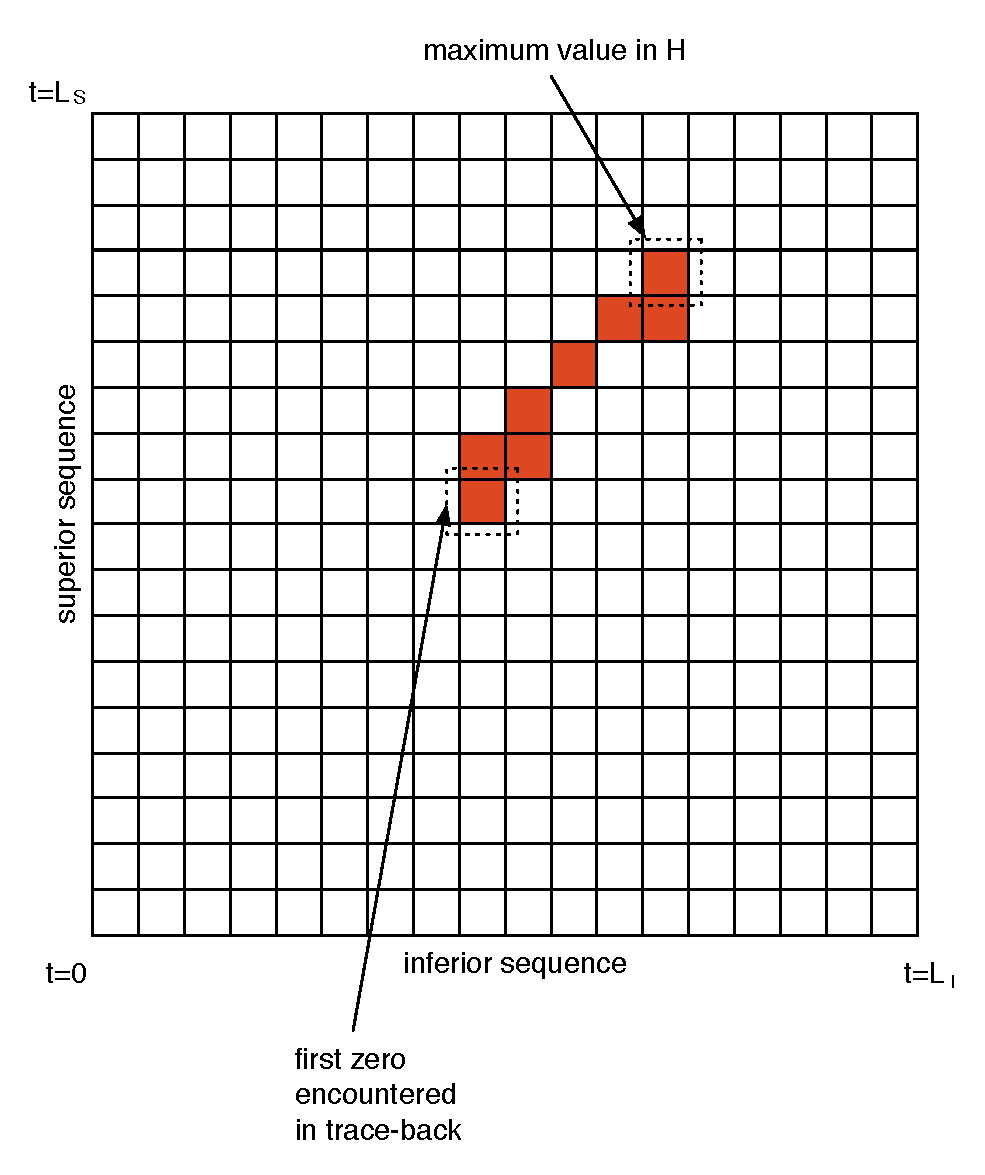
\includegraphics[scale=0.75]{SICSW_1}
\caption[Finding Optimal Subsequence]{The optimal local alignment ends with the maximum value of H. Once it has been found, we trace backwards (either below, to the left, or diagonally down and to the left) along the maximum values encountered until we find a $0$, which marks the beginning of the local alignment.}
\end{center}
\end{figure}
\\
\item Calculate the aligned-Euclidean distance over all aligned vectors found in step 1 and store this along with the length of the aligned vector sequences.
\end{enumerate}
This is where DPLA utilizing the Smith-Waterman algorithm ends, because it is only concerned with the best local alignment. As stated previously, we also are interested in this alignment, but we must continue to search for other subsequence alignments between what is left in our superior sequence and the entirety of our inferior sequence. Therefore, we continue on with the following steps:
\begin{enumerate}
\setcounter{enumi}{2}
\item Remove the submatrix from $H$ that corresponds to the superior sequence's subsequence used in the alignment found in step 1 and store this in H (see Figure 26).
\begin{figure}[h!]
\begin{center}
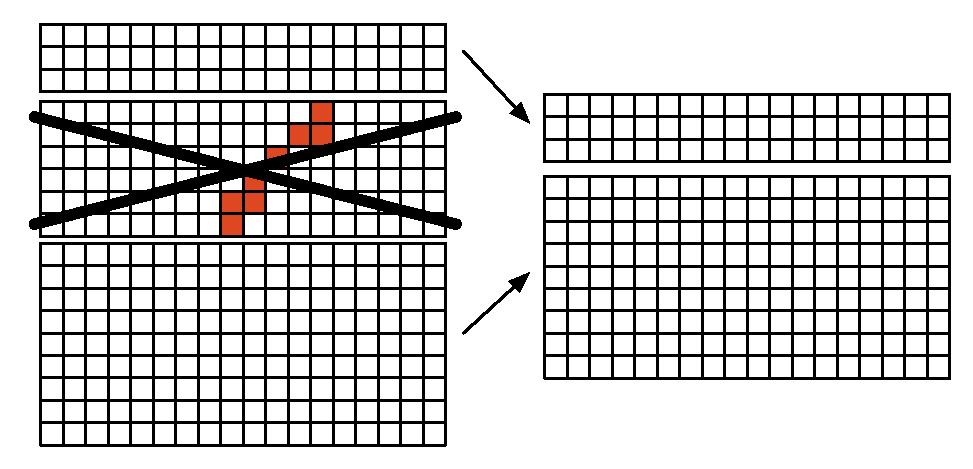
\includegraphics[scale=0.8]{SICSW_2}
\caption[Removing Optimal Subsequence]{After the aligned-Euclidean distance is calculated for the optimal local alignment, the superior's subsequence involved in that alignment is removed.}
\end{center}
\end{figure}
\\
\item Repeat steps $1-3$ until there are no longer any values in H above 0.
\item Calculate the sum of all distances generated in the various passes through step 2 and divide by the sequence length of the superior sequence to normalize for sequence length.
\end{enumerate}
This process will give us a preliminary value for the ${ICSW}$ distance in one direction (e.g. where $Z^1$ is treated as the superior sequence and $Z^2$ the inferior):
\begin{equation}
D_{ICSW_{S \to I}}^{(Prelim)} = \frac{\sum_{j=1}^J \sum_{k=1}^{K(j)} \sqrt{ \sum_{l=1}^L (A_{jkl}^1 - A_{jkl}^2)^2}}{L_S}
\end{equation}
where $D_{ICSW_{S \to I}}^{(Prelim)} $is the preliminary $ICSW$ distance from superior sequence $S$ to inferior sequence $I$, $J$ is the number of subsequences chosen for alignment, $K(j)$ is the length of the $j$th subsequence pair, $L$ is the dimensionality of our timbre vector, $A_{jkl}^1$ is the $l$th element of the $k$th vector in the $j$th aligned subsequence taken from $S$, $A_{jkl}^2$ is the $l$th element in the $k$th vector in the $j$th aligned subsequence taken from $I$, and $L_S$ is the length of $S$.

Once we calculate our preliminary I-CSW distances in both directions, we penalize the alignment combinations chosen by scaling the preliminary distances in the following ways:
\begin{itemize}
\item If alignments are not ordered appropriately in time (i.e. if the aligned subsequences do not progress forward in time for both sequences) then the appropriate I-CSW distance is scaled by the minimum number of subsequence swaps required to order the inferior sequence's segments plus the number of aligned subsequences, all divided by the number of aligned subsequences (see Figure 27). 
\begin{figure}[h!]
\begin{center}
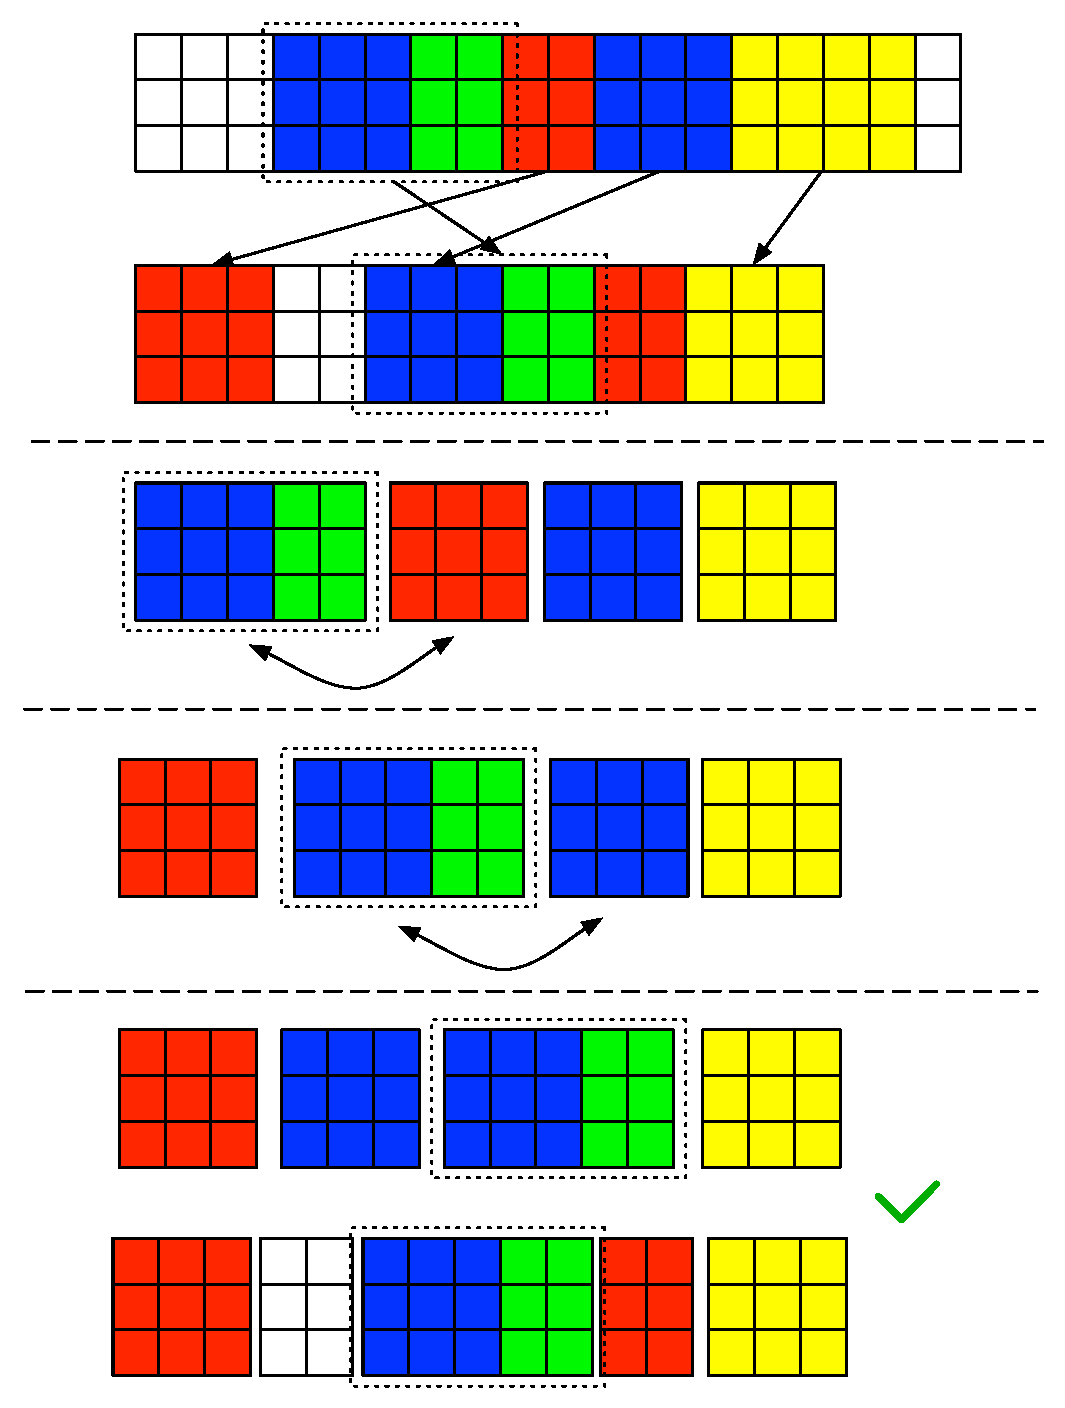
\includegraphics[scale=0.7]{Penalty_1}
\caption[Penalizing Swaps]{Two swaps are necessary to return the progression of aligned subsequences from the inferior sequence back to its original ordering.}
\end{center}
\end{figure}
\\
This value is therefore at least one (which occurs when the segments are appropriately aligned as they are). In other words, if the number of necessary subsequence swaps is $N_S$ and the total number of subsequences is $N_T$, the penalty multiplier will be:
\begin{equation}
P_{SWAP} = \frac{N_S+N_T}{N_T}
\end{equation}
\item Any overlap in the segments chosen from the inferior sequence are treated by determining whether their inclusion causes for more overlap than their exclusion causes for a gap between segments. If the overlapped segment causes for more overlap when included than gap when excluded, it is flagged as a `repetition' and dealt with separately (see next item). Once repetitions have been removed, the cumulative overlap and cumulative gap amounts are summed over the length of the entire sequence, added to the inferior sequence length, and then divided by the inferior sequence length, and this value is used to further scale the distance (see Figure 28). 
\begin{figure}[h!]
\begin{center}
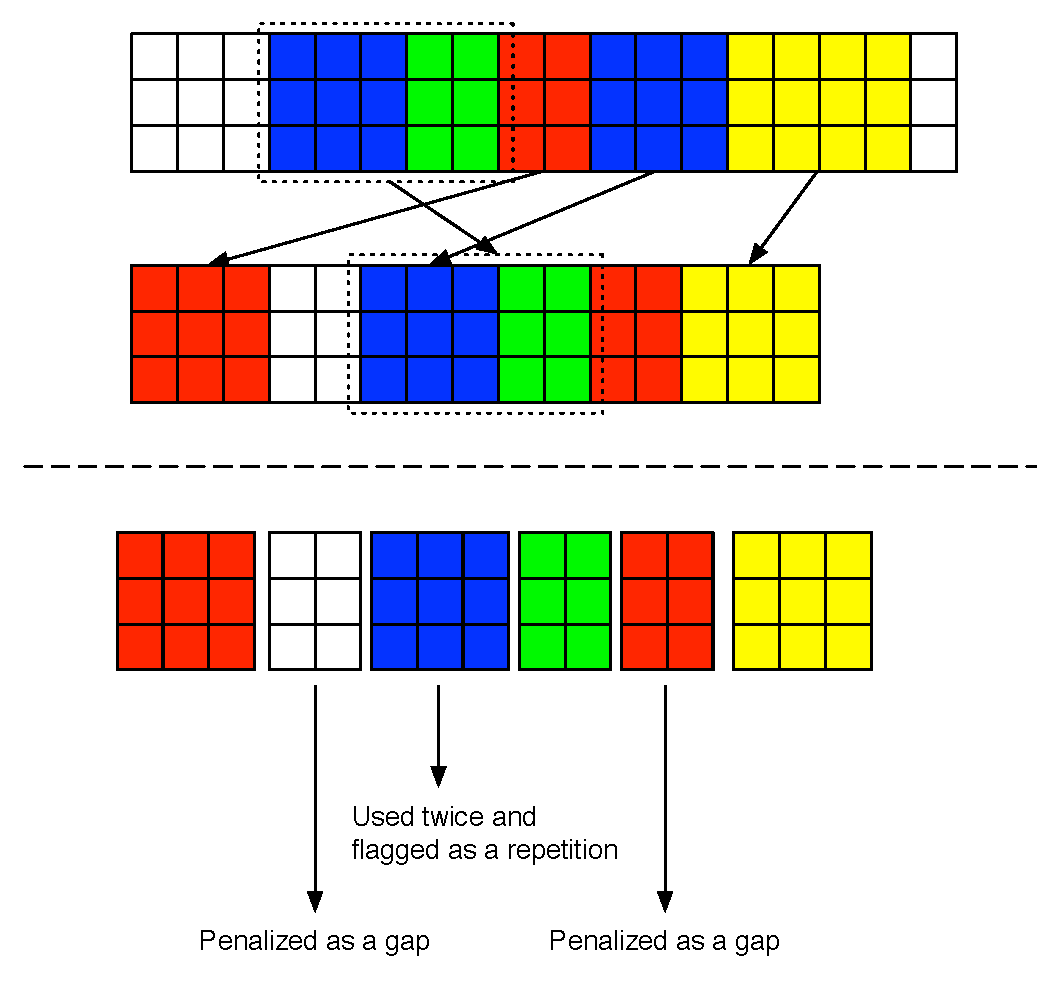
\includegraphics[scale=0.7]{Penalty_2}
\caption[Penalizing Swaps]{The blue region is used twice by the superior sequence and is marked as a repetition, not to be penalized here. However, the two 2-vector gaps are penalized.}
\end{center}
\end{figure}
\\
This value is also at least one. If $L_O$ is the cumulative overlap, $L_G$ is the cumulative gap, and $L_I$ is the total length of the inferior sequence, the penalty multiplier will be:
\begin{equation}
P_{O/G} = \frac{L_O+L_G+L_I}{L_I}
\end{equation}
\item If any repetitions are extracted from the previous overlap/gap distance adjustment, they also affect the distance measurement, but to a lesser degree than an overlap, since repetition of a lengthy subsequence should not penalize the similarity of timbal evolution to a large degree. We penalize the distance measure by counting the number of repetitions, adding by the number of total subsequences extracted, and dividing by the number of subsequences extracted to give us a repetition adjustment scaling factor. If the number of repetitions is $N_R$, the penalty multiplier will be:
\begin{equation}
P_{REP} = \frac{N_R+N_T}{N_T}
\end{equation}
In the example in Figure 28 there is only one repetition of six total subsequences aligned, producing a $P_{REP}=(6+1)/6=7/6$.
\end{itemize}
The three scaling factors mentioned above are all used to adjust the preliminary I-CSW distances calculated in each direction (from sequence $Z^1$ to $Z^2$ and $Z^2$ to $Z^1$):
\begin{equation}
D_{ICSW_{S \to I}} = D_{ICSW_{S \to I}}^{(Prelim)} * P_{SWAP} * P_{O/G} * P_{REP}
\end{equation}

The two resultant I-CSW distances are then summed together to provide the SI-CSW distance ($D_{SICSW}$), which, as previously shown, is used to calculate our timbre sequence similarity measure, $S_T$.

It should be noted that our approach is still greedy in that we optimize local alignments without regard to how it will affect our overall global scores (i.e. we optimize before applying our scaling factors), but we believe it to be a considerable upgrade over typical DTW and non-time warped aligned-Euclidean methods. A more systematic and less greedy measure is left for future work.

In order to test our approach versus the three approaches discussed above (aligned-Euclidean, global DTW, and DPLA), we developed a controlled experiment that starts with a sound and applies various kinds of temporal distortion that should not alter its timbal similarity score. The distortions applied are broken into the following categories:
\begin{itemize}
\item Slight global time scaling (randomly selected between $2-5\%$) combined with time shifting (randomly selected between $100-500ms$).
\item Local time warping (randomly selected such that the warping path does not diverge from the diagonal more than 5 frames).
\item Random sample deletion (randomly selected and totalling between $2-5\%$ of all content).
\item Random extension of stable timbral content randomly selected and totalling between $2-5\%$ of all content. 
\end{itemize}
We measure how invariant each model is to these temporal distortions by considering a nonzero distance between the original sample and one of its distorted versions as an error. We measure these errors given a number of different sample files and average over each distortion.

We then progressively distort our target in way that produces sounds that we would like to consider less and less timbrally similar by:
\begin{itemize}
\item Introducing new timbal content (between $10-50\%$ of the file length) while randomly deleting other content.
\item Re-ordering random subsequences within content (by choosing subsequences that are between $10-20\%$ of the file length and swapping out of order up to 5 times).
\item Randomly inserting repetitions paired with random deleting of non-repetitive segments (by choosing subsequences that are between $10-20\%$ of the file length and repeating up to 3 times).
\item Applying severe temporal warpings (randomly selected such that the warping path diverges at least more than 10 frames once during the length of the file). 
\end{itemize}
In these cases, we want the amount of distortion severity to be inversely proportional to the similarity calculated. We therefore measure how the similarity calculated changes as a function of increased distortion severity. For example, we look at the rate at which the similarity measure decreases as the introduction of new timbal content increases from $10-50\%$ of the file length.

\subsubsection*{3.2.2 Genetic Operator Variations}
In order to implement a genetic algorithm within an automatic programming framework, one needs to develop an appropriate representation of each program, which we have done in section 3.1.2. This representation allows us to represent all programs as a set of trees. However, this is not enough to define an input space. In order for a set to become a space, a topological ordering must be placed on the elements. This ordering will inform the shape of the objective landscape (i.e. fitness function) and therefore directly influence the difficulty of search through the space for some desired solution. In algorithm space, such orderings are typically not made explicit due to its complexity. Instead, implicit orderings are acquired via the operators used to search the space (da Silva, 2008, p. 102). Thus, using different operators will result in different input-space orderings. The goal is to find the input-space ordering that makes the objective landscape as �searchable� as possible. This can be measured via the negative slope coefficient (NSC), developed by Vanneschi (2004, p. 54).

The NSC is computed by first generating a fitness cloud, where one plots the fitness of an individual by the fitness of one of its neighbors (children in GP parlance). The shape of this cloud provides some intuition of the evolvability of the genetic operators used and thus some intuition about the difficulty of the problem using these operators (Vanneschi, 2004, p. 130). It is important to note that Vanneschi found that uniform random sampling of individuals to use in the generation of the fitness cloud typically results in generating individuals whose fitnesses tend towards the lower end of the fitness range and therefore does not give a complete picture of how fit neighbors are for individuals throughout the entire fitness spectrum (2004, p. 132). Instead, Vanneschi suggests using the `Metropolis-Hastings' sampling technique, which have adopted in our work. For pseudo-code explaining the technique see (Vanneschi, 2004, p. 131).

Vanneschi also notes that choosing an appropriate neighbor from an individual (via that application of a genetic operation) is only useful if that neighbor would not be immediately discarded via the selection mechanism. Therefore, Vanneschi suggests that neighbors are found via a Tournament Selection (see Section 3.2.5) process that we also have adopted, where $k$ randomly generated neighbors enter a tournament and the winner is chosen as the neighbor to use in the fitness cloud. Following Vanneschi's suggestion, we will choose only one neighbor per individual, which will be selected as the winner of a tournament of size $k=10$.

The NSC is calculated by partitioning the x-coordinate of the scatterplot into M segments of the same length and then dividing the y-coordinate into the ranges spanned by each x-segment. The average x and y values are calculated in those regions and a piecewise linear function is generated through those points. The slopes of the piecewise segments are calculated and only the negative values are summed to provide the NSC. In other words, for each segment $S_i$, the slope $P_i$ is calculated in the following way:
\begin{equation}
P_i = \frac{N_{i+1}-N_i}{M_{i+1}-M_i}
\end{equation}
where $M_i$ is the average of the original individuals' fitness values within the $i$th partition and $N_i$ is the average of the selected neighbors' fitness values within the $i$th partition. The NSC is calculated from these slopes as:
\begin{equation}
NSC = \sum_{i=1}^{M-1} max(0, P_i)
\end{equation}
If $NSC = 0$, the problem is considered easy, if $NSC < 0$ it is difficult, and the value of NSC quantifies this difficulty (p. 139). In our experiments, we have chosen $M=10$ so that we can generate enough points per segment of the fitness cloud given a relatively small sample size of $1000$ for the average values to be descriptive of the segment.
The genetic operations we have decided to test are the most common set found in GP problems. A brief description of each follows:
\begin{description}
\item [Crossover] - In crossover, two trees are selected at random within the population, a subtree from each is selected and removed, and then the subtrees are attached to the cut points of the opposite trees. When ensuring syntactic correctness through the search process, the crossover operation must make sure to only choose subtrees that can be swapped and still result in syntactically correct structures (see Figure 29). 
\begin{figure}[h!]
\begin{center}
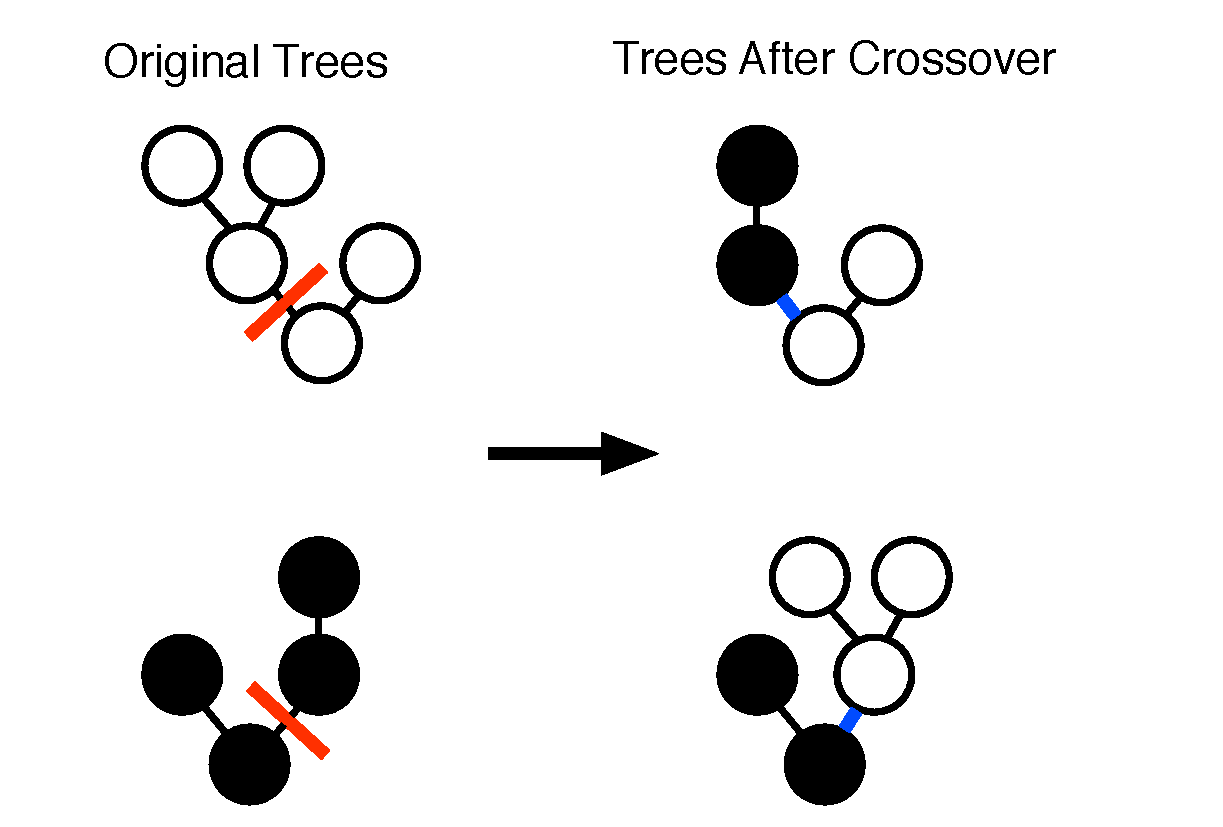
\includegraphics[scale=0.5]{Crossover}
\caption{Tree crossover with the root (i.e. dac\texttildelow{} below the terminals).}
\end{center}
\end{figure}
\\
\item[Subtree Mutation] - This, unlike Crossover, is a unary operator, which removes a subtree at a random location within a tree and replaces it with a randomly generated subtree. As with crossover, syntactic rules must be enforced during generation of this new subtree (see Figure 30).
\begin{figure}[h!]
\begin{center}
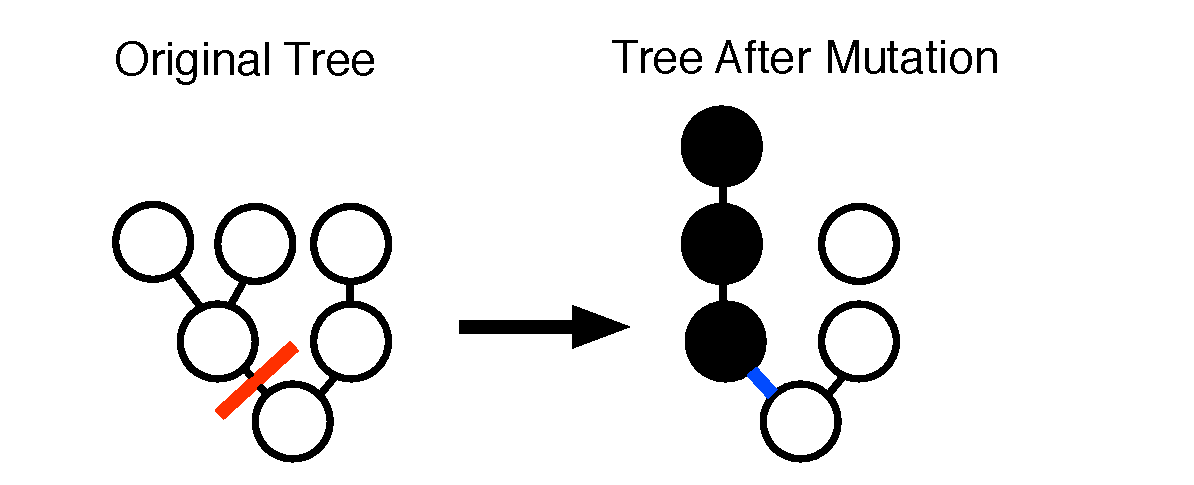
\includegraphics[scale=0.5]{SubtreeMutation}
\caption{Subtree mutation with the root (i.e. dac\texttildelow{} below the terminals).}
\end{center}
\end{figure}
\\
\item[Point or Node Replacement Mutation] - Instead of removing an entire subtree and replacing it with a randomly generated subtree, Point Mutation randomly removes a single node in a tree and replaces it with a node that is syntactically valid in that position (i.e. with the same number of inputs and the same input/output types) (see Figure 31).
\begin{figure}[h!]
\begin{center}
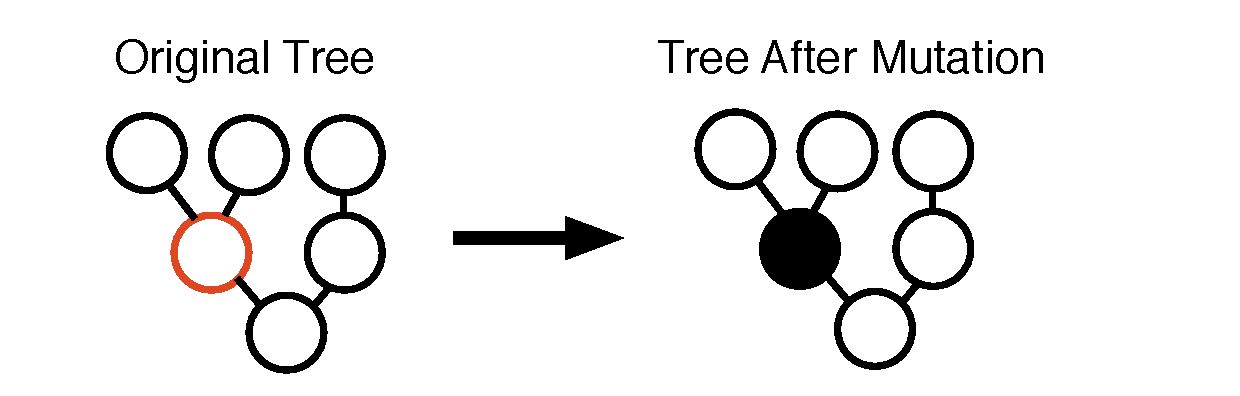
\includegraphics[scale=0.5]{PointMutation}
\caption{Point mutation with the root (i.e. dac\texttildelow{} below the terminals).}
\end{center}
\end{figure}
\\
\item[Reproduction] - This is the simplest of all genetic operators in that it is simply a pass-through mechanism for selected patches. Reproduction allows for highly fit individuals to remain in the population from generation to generation so that they may be involved in crossover with other individuals (and so they can be continuously mutated) in the hope that a higher fit individual will result (see Figure 32).
\begin{figure}[h!]
\begin{center}
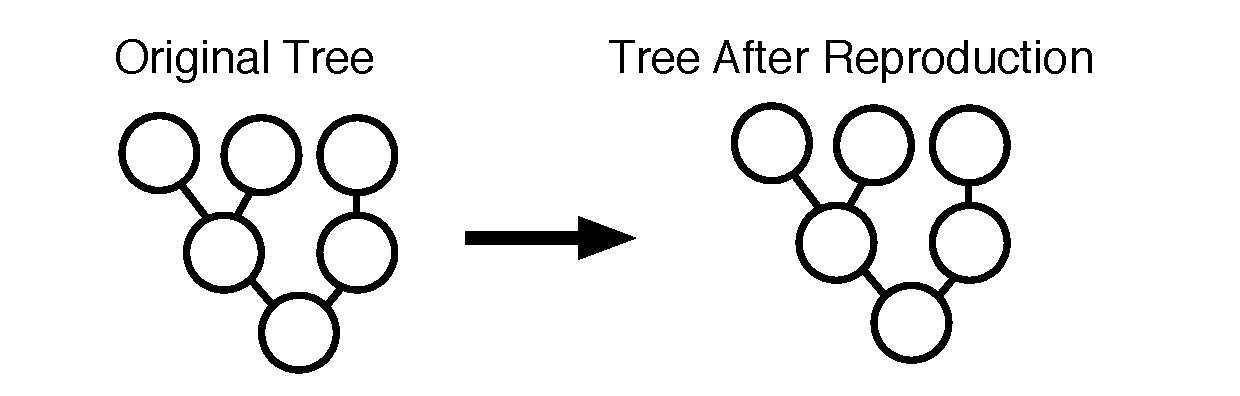
\includegraphics[scale=0.5]{Reproduction}
\caption{Reproduction with the root (i.e. dac\texttildelow{} below the terminals).}
\end{center}
\end{figure}
\\
\end{description}

We have decided to use the following combinations of genetic operators (and proportions of how many patches undergo each operation in the combination) and have tested their ability to simplify the search problem using NSC:

\begin{itemize}
\item 75\% Crossover, 25\% Subtree Mutation
\item 75\% Crossover, 25\% Point Mutation
\item 25\% Crossover, 75\% Subtree Mutation
\item 50\% Crossover, 25\% Subtree Mutation, 25\% Point Mutation
\item 50\% Crossover, 25\% Subtree Mutation, 25\% Reproduction
\item 25\% Crossover, 50\% Subtree Mutation, 25\% Reproduction
\end{itemize}
As previously mentioned, each of these tests will consist of generating $1000$ patches using the Metrpolis-Hastings sampling technique and selecting one neighbor for each of these patches from the winner of a Tournament Selection process involving $10$ randomly generated neighbors in a manner consistent with the combinations listed above.
\subsubsection*{3.2.3 Target Sound Selection}

The previous discussion has provided a means to develop an appropriate fitness function for our problem and an input space that makes its corresponding fitness surface (given the pre-defined fitness function) as easily-searchable as possible within the GP framework. Going forward, we want to make sure that what we are testing is the appropriateness of our search technique over this space and corresponding fitness surface and not the appropriateness of or ability for sounds to to actually be realized in Max. For example, there may be time-varying timbres that require tens of thousands of Max objects to replicate perfectly.

As Mitchell and Creasey point out in their work on sound matching via evolutionary methods, the difficulties in obtaining an optimal solution to a complex search problem are based on several factors, only one of which is the search algorithm itself (2007, p. 1). They recommended using a `contrived' target in order to test only the efficacy of the search. In our problem domain, a contrived target refers to one that was generated by a known synthesizer (i.e. Max patch). Mitchell and Creasey suggest randomly generating contrived targets using points uniformly spread out in the input-space (p. 2). If the search algorithm is able to match all of the contrived targets with a good spread in the input space, it is suggested that one can then assume it will be able to match any target (p. 2). This assumes however that a uniformly spread set of points in the input space will map to a large area of the timbre space, which is not necessarily the case.

We therefore have chosen to test the search algorithm on three contrived targets with varying degrees of complexity in order to attain an understanding of the limitations of the search algorithm (see Figure 33). Since these contrived targets are realizable in the Max environment, they should be found given an intelligent enough search. While it is important that these targets are sufficiently spread out in the input space in order to promote some sense of generalization of the search technique through this space, we later test the search technique using non-contrived targets in order to provide a more resounding argument for this (as is discussed in 3.2.7).

We are able to measure success in two different ways when using contrived targets and will speak to both in the results section whenever our tests involve them:
\begin{enumerate}
\item We are able to compare the topographies of the contrived-target patch and the best-of-run patch that is generated during the search process. If the topographies are exact matches, we must consider this an outright success. However, if different, the topologies provide intuition about how code bloat enters the search, how well the topologies of local optima mirror the target topology (i.e. if there is a correlation between timbre and topology space), and how well different topologies can mimic the timbre produced by a contrived-target topology (i.e. how realizable is the target timbre given topologies that differ from the topology that generated the target).
\item We are able to measure the best-of-run fitness and determine how well our search is able to achieve its goal of finding a patch that can produce the target timbre.
\end{enumerate}

\subsubsection*{3.2.4 Limiting Code Bloat and Promoting Parsimony}

By using contrived targets and objects that are able to construct them perfectly, we have set up a self-fulfilling prophecy of sorts that would rarely be encountered in practice. It is important to look at how our solutions degrade (or the time it takes to find an optimal solution increases) once the object set grows beyond the necessary set of objects and/or necessary objects are removed from the object set. However, before these parameters are varied, we look at other sorts of resource limitations that have proven effective in other GP research to see if they are useful in this problem space. We are able to focus on the efficacy of these methods and provide appropriate comparisons if we tightly control our experiments in the way suggested.

In the Prior Work section, we listed a number of methods for limiting the region of input space we search including: Enforcing strong typing constraints, applying either static (SMTD) or dynamic maximum tree depths (DMTD), and/or enforcing limitations on the total amount of resources in a given population using either resource limited GP (RLGP) or dynamic resource limited GP (dRLGP) constraints. These methods were developed to be used for any problem domain and only discriminate against solutions that are not parsimonious or syntactically valid. They promote efficiency and low storage requirements as well as controllability of the resulting algorithms due to their propensity to generate low-dimensional parameter sets. However, as with any kind of limitation of the searchable input space, we must make sure not to exclude possible solutions. Therefore, a fine balance must be found between the improvements in the efficiency of the search (i.e. iteration count to the optimal solution) and the decrease in fitness of the optimal solution found. Since we can be sure that all solutions are attainable for our contrived targets and associated object sets, we can fairly compare different severities of limitation across all targets.

A brief recount of each limitation follows:

\begin{description}
\item [Static Maximum Tree Depth (SMTD)] - Throughout the entire search process, a static limit is placed on the maximum tree depth of each individual's representation.
\item [Dynamic Maximum Tree Depth (DMTD)] - Throughout the search process, the limit placed on the maximum tree depth is increased in order to slowly evolve more and more sophisticated (i.e. complex) algorithms.
\item [Resource Limited GP (RLGP)] - Throughout the entire search process, a static limit is placed on the number of resources (i.e. the sum of function and terminal nodes) used in an entire population. This limit is therefore applied to the overall population as opposed to SMTD and DMTD, which is applied to each individual in a population.
\item [Dynamic Resource Limited GP (dRLGP)] - Throughout the search process, the limit placed on the amount of resources available to a population increases in order to slowly evolve more and more sophisticated algorithms.
\end{description}

To test the effects of these limitations, we use the contrived target set, apply these limitations at various severities, and calculate both how error increases (i.e. how fitness decreases) as a function of the amount of limitation as well as how quickly solutions can be found as a function of the amount of limitation. This analysis provides us with an optimal degree of limitation that balances both an increase in efficiency with a decrease in accuracy.

Since we have not yet discussed nor tested how best to initialize our population, nor how we should select individuals to undergo genetic operations to produce each successive generation, we choose to use the most common methods for these tests, Grow Initialization and Fitness-proportionate Selection (see Section 3.2.5), and improve upon these (if improvements are possible) in separate testing. On each permutation of the aforementioned limitation, we are interested in recording the fitness of the best-of-run individual, the iteration/generation in which that individual was created, the total number of iterations in each run, and the trends of average fitness of each generation, maximum fitness in each generation, and minimum fitness in each generation, so that we can analyze how quickly solutions are found, how good they are, and whether or not the various trends mentioned seem to level off by the time the last generation is assessed. In our testing, we run tests while imposing each of the following search space limitation constraints over $200$ iterations of $100$ individuals, for each of the contrived targets:
\begin{itemize}
\item A SMTD of $4,5,6,7, \text{and }8$.
\item A DMTD between $4-6$, $6-8$, and $4-8$ with the limit increasing at equal steps along the $200$ iterations.
\item A RLGP of $1000, 2000, 3000, 4000, \text{and } 5000$.
\item A dRLGP between $1000-3000$, $2000-4000$, and $1000-5000$ with the limit ramping up linearly over the $200$ iterations.
\item A SMTD of $5$ and a RLGP of $2000$ and SMTD of $8$ and a RLGP of $5000$.
\item A DMTD between $6-8$ and a dRLGP of $2000-4000$ and DMTD of $4-8$ and a dRLGP of $1000-5000$.
\end{itemize}

\subsubsection*{3.2.5 Initial Conditions and Selection Methods}

Along with algorithm representation and operator selection, the population initialization and selection mechanisms form the basis of the GP architecture. It may seem strange to first look at limiting code bloat and promoting parsimony before exploring these fundamental GP mechanisms. We have chosen this ordering because of the benefits reducing code bloat and promoting parsimony provides to all testing that follows it. Testing of the remaining parts of our system requires full test runs. By applying the mechanisms explored in the previous section, these test runs will be able to run more efficiently by not looking in regions of the input space that we are not interested in (i.e. those that would produce syntactically invalid Max patches or those whose solutions would be complex and likely unable to run in Max in real time, which is a desirable properly of any synthesis algorithm).

The three initialization flavors we study are Full, Grow, and Ramped Half-and-Half initialization. A brief description of each of these methods follows:
\begin{description}
\item [Full Initialization] - The root node is chosen and then, in a depth-first fashion, function nodes are added until the maximum tree depth is reached, at which time a terminal node is chosen. This process is repeated for all branches, resulting in a full tree where each branch meets the maximum tree depth. The risk of using full initialization is that one may start with a population where individuals are too similar (given that they are all full tree structures).
\item [Grow Initialization] - This is very similar to Full initialization, except that as the branches are being built, each node is selected from the pool of both function and terminal nodes. The result is a tree with branches that are no greater than the maximum tree depth, but that may be shorter (due to a terminal node being chosen before the maximum depth is reached). The risk of using Grow initialization is that it may result in a population with too many individuals that have terminated prematurely and are therefore too simple to perform any meaningful function.
\item [Ramped Half-and-Half Initialization] - This is the most common form of initialization in Genetic Programming. It uses Full initialization for half of the individuals in the population and Grow initialization for the other half. It also increases the depth limit for both methods as the population grows in size. The ramping of the depth limit along with using both Full and Grow methods produces a wide variety of patches in shape and size.
\end{description}

The four selection methods we have chosen are known as Fitness-Proportionate, Ranking, Tournament, and Double Tournament. A brief description of each of these methods follows:
\begin{description}
\item [Fitness-Proportionate Selection] - Individuals from one generation are chosen to populate the next generation with probability proportional to their fitness. Thus, the more fit an individual is, the more likely it will be chosen to breed new individuals for the next generation. In figure 34, the top row of squares represent the individuals in a population and the pie chart below represents their respective fitnesses as fractions of the sum of all fitnesses in the population. In other words, for fitness-proportionate selection, the pie chart illustrates the probability with which each individual will be selected to breed the next population. Note in the figure that the red and green individuals from this example are chosen twice due to their high fitnesses (i.e. probabilities of selection), while the yellow is not chosen due to its low fitness.
\begin{figure}[h!]
\begin{center}
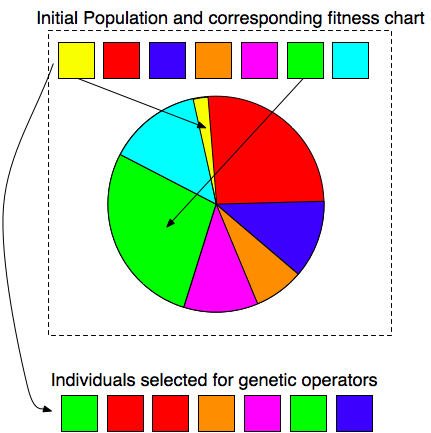
\includegraphics[scale = 0.7]{PieChartSelection}
\caption{Fitness-proportionate selection}
\end{center}
\end{figure}
\\
\item [Ranking Selection] - In ranking selection, individuals from one generation are ranked in order from least to most fit and the probability of selection is proportional to this ranking. For example, if there are $N$ individuals in a generation, then the least fit individual has rank $1$ and the most fit rank $N$. The sum of all ranks is $N*(N+1)/2$. Therefore, least fit individual will have a selection probability of $1/(N*(N+1)/2)$ or $2/(N*(N+1))$ regardless of its fitness value and the most fit individual will have a selection probability of $N/(N*(N+1)/2)$ regardless of its fitness value. 
\item [Tournament Selection] - In tournament selection, a set of patches are selected at random from a generation and the most fit of those patches is selected. All patches are placed back in the pool of all patches to be randomly sampled from on the next iteration. This random sampling of patches and the tournament that follows is repeated as many times as there are individuals to be selected.
\item [Double Tournament Selection] - In Double Tournament selection, each individual chosen to be part of a tournament is already the winner of a tournament with different conditions. The most common Double Tournament Selection mechanism works by first choosing a random grouping of patches, selecting the most parsimonious of those patches with probability $D$, and placing the winner in a pool of other parsimony tournament winners to be involved in a fitness tournament. The idea is that Double Tournament Selection applies parsimony pressure absent from typical Tournament Selection, which is useful for controlling code bloat. The most common tournament size for the parsimony tournament is two with $D = 0.7$ and the most common tournament size for the fitness tournament is seven (Luke \& Panait, 2006, p. 21).
\end{description}

We have chosen to enumerate the various combinations of initialization and selection mechanisms as it is unclear exactly how correlated these two mechanisms are in producing an optimal search algorithm. We are interested in determining how the best-of-run average fitness error over all contrived targets varies as we test these combinations as well as how they affect the resultant algorithm complexity (measured as the size of the topology of the best-of-run patch). Therefore, for each tested combination of initialization mechanism and selection mechanism, we record these values and compare. Again, our tests will involve moving through $200$ iterations of $100$ individuals. The combinations we test are listed below:
\begin{itemize}
\item Full initialization and Fitness-Proportionate Selection.
\item Full Initialization and Ranking Selection.
\item Full Initialization and Tournament Selection.
\item Full Initialization and Double Tournament Selection.
\item Grow Initialization and Fitness-Proportionate Selection.
\item Grow Initialization and Ranking Selection.
\item Grow Initialization and Tournament Selection.
\item Grow Initialization and Double Tournament Selection.
\item Ramped Half-and-Half Initialization and Fitness-Proportionate Selection.
\item Ramped Half-and-Half Initialization and Ranking Selection.
\item Ramped Half-and-Half Initialization and Tournament Selection.
\item Ramped Half-and-Half Initialization and Double Tournament Selection.
\end{itemize}
We aim to strike a balance between algorithm complexity and fitness so as to provide the user with a controllable architecture (i.e. one with a small number of variable inputs) and therefore choose an initialization/selection mechanism combination that allows us the best trade-off. This selection along with the choices made given the aforementioned tests will provide us with an optimal base GP architecture. The following tests seek to augment this architecture and provide further evidence that it will generalize well to all timbres.

\subsubsection*{3.2.5.2 Non-standard Selection Methods}

Aside for the above methods of patch selection for the subjection to genetic operations, we referred to three other non-standard flavors of mechanisms involved in the selection process in the Prior Work section that have shown to be useful for certain GP problems:

\begin{enumerate}
\item Using the \textbf{Parallel and Distributed Genetic Programming (PADGP)} paradigm, where subpopulations within the GP population are formed and individuals between populations are rarely allowed to interact, such that the subpopulations are allowed to evolve independently. The parameters to this model are the communication topology between subpopulations (i.e. whom transfers individuals to whom), the number of subpopulations, the number of individuals per subpopulation, the frequency of exchange of individuals, and the number of individuals exchanged (Vanneschi, 2004, p. 178). The three communication topologies used in the literature are the ring topology (where the subpopulations form a circle and each passes individuals in a clockwise manner), the grid topology, (where subpopulations form a grid and each population sends and receives individuals from all four neighbors), and the random topology (where each subpopulation sends individuals and receives individuals from exactly one random subpopulation different from itself at each migration period).
\item Applying \textbf{Simulated Annealing (SA)} on the parameter set of each patch in a population to find the optimal parameter set for the given patch topology before running the patches through the selection process.  
\item Starting with a more lenient fitness function that the selection mechanism is aware of and making it more demanding over the lifecycle of the search, such that only in the last few iterations is the appropriate fitness measure applied before selection. The set of fitness functions involved are formally referred to as \textbf{Increasingly Discriminating Fitness functions (IFFs)}. 
\end{enumerate}

We believe our treatment of this problem would not be complete if we did not ascertain whether these more modern GP mechanisms could be helpful to us. The above approaches attempt to provide a more efficient means to achieve an optimal solution and we therefore test them on this ability. We calculate statistics on how quickly (i.e. how few iterations) we are able to perform in order to find a near optimal solution. In the case of using SA in combination with GP, it is not immediately clear how to directly compare this strategy with standard GP, due to the internal iterations SA proceeds through within each GP iteration. In this case, the number of algorithms searched (i.e. translated into the Max environment for audio processing) will be used for a fair comparison.

In our testing involving PADGP, we follow Venneschi's suggestion to use a random communication topology, a frequency of exchange of every ten generations, and a population exchange size of $10\%$ of the total number of individuals in each subpopulation (Vanneschi, 2004, 190). We test this method using $200$ iterations of $100$ individuals, where the $100$ individuals are split into $5$ groups of $20$.

In testing Simulated Annealing on the parameter set of each patch in a population between generations, we limit the system to search through as many individuals as we are in a typical run (i.e. $20,000$). If we allow each patch to undergo $10$ SA iterations, this reduces the number of iterations of GP to $20$. We do not want to limit the ability of our system to utilize GP and we feel that $20$ is possibly just enough iterations to leverage it, so we keep the SA iteration count at $10$. SA is a simple strategy that generates a random neighbor, calculates its fitness and a corresponding `acceptance probability' given that fitness and the fitness of the current individual, compares the probability to a uniformly randomly chosen number, and makes the neighbor the new individual to run SA on if the probability is greater than the random number chosen. As the iteration count increases, the acceptance probability becomes more and more strict for poorly performing individuals. As is standard, we will use the Metropolis-Hastings algorithm to choose neighbors (where a neighbor in this context is a patch with the same exact topology, but where a single parameter is changed by no more than $50\%$ of its magnitude) and will assume an acceptance probability of:
\begin{equation}
P(S_{T_{p_1}}, S_{T_{p_2}}, T) = \left\{
   \begin{array}{l l}
    1 & \quad \text{if $S_{T_{p_2}}>S_{T_{p_1}}$}\\
    e^{-(S_{T_{p_2}} - S_{T_{p_1}})/T} & \quad \text{if $S_{T_{p_2}}\leq S_{T_{p_1}}$}
    \end{array} \right.
\end{equation}
where $S_{T_{p_1}}$ and $S_{T_{p_2}}$ are the similarity scores for some patches $p_1$ and $p_2$, and $T$ is the `temperature value', which will range from $1-10$ over the ten iterations (Kirkpatrick, Gelatt, and Vecchi, 1983, p. 673).
\subsubsection*{3.2.6 Expanding/Restricting the Searchable Region of Input Space}

After the controlled experiments from above - meant to compare variations of each GP mechanism against one another - have been performed, it is appropriate to move away from the perfectly contrived examples we have used so far. Stepping away from these tests towards a `real-world' scenario involves two steps:

\begin{enumerate}
\item We will both expand and contract the object and parameter (by discretizing with greater and less resolution) sets used to generate Max patches when searching for our contrived targets. By looking at how well (or how quickly) our solutions approach the contrived Max patches, we will be able to show how robust our system is to starting with an inappropriate resource set (i.e. one with objects that are not involved in the optimal solution and/or with necessary objects in the optimal solution not present). Even if the system is given a timbre that was produced (or is easily producible) by a Max patch, it is likely any object set we choose for our system to source from will not contain all of the objects (and only the objects) necessary to build the target. Since a `real-world' timbre may not even be realizable with 100\% percent accuracy in the Max environment, these tests are not enough to show how well our system will generalize to all timbres. However, they are a good first step towards that goal and provide us with more information (namely, the patch topologies of both the target and the solution to compare) to use to assess the robustness described.
\item The final step towards showing system generalization over all timbres involves using timbres that are not contrived. This is discussed in the next section (3.2.7 Generalization).
\end{enumerate}

In order to test how well our system performs given object and parameter sets that are either not sufficient or over-complete, we look at how well our performance drops off as we restrict or expand our object and parameter sets over our contrived examples. We have chosen to use the following sets for each example in our tests:

The important data we gather from tests include how the best-or-run patches' fitnesses decrease as we change the cardinality of the function set away from only containing necessary functions and as we change the possible parameter values that functions may take, as well as recording how the iteration count required to reach a best-of-run patch varies given changes in these variables.

\subsubsection*{3.2.7 Generalization}
It is necessary to test this system on a number of real-world sounds in order to gauge its ability to generalize to sounds that are not contrived. As Riionheimo and Valimaki note, ``the quality of resynthesis of real recordings is more difficult to measure as there are no known correct parameter values'' nor synthesis topologies (2003, p. 13). In genetic programming research where a known target algorithm does not exist, the performance of the system is usually measured using the fitness level at which the system converges and how long it takes to converge to that level. We do not have a known topology for such real-world examples and therefore must only use this measure to determine how successful our search method is. In order to determine how well our search generalizes over all real-world sounds, we have chosen five different target sounds ranging from those generated by music instruments to those generated in nature. A brief description of the timbres we have chosen follows:
\begin{itemize}
\item
\item
\item
\item
\item
\end{itemize}
We have searched for these timbres using the optimal parameters/methods obtained in the previous tests, varying a stopping criteria based on iteration count - with runs ending at $200$, $400$, $600$, and $800$ iterations - and a fitness threshold (which is based on the results of the timbre similarity tests). We have calculated the typical statistics (min, max, mean) over each stopping criteria variation for each individual target as well as all targets combined. The results of these tests can be found at the end of \textbf{Chapter 4 - Results} with an accompanying discussion.

\newpage
\end{flushleft}
\end{document}